% ****** Start of file aipsamp.tex ******
%
%   This file is part of the AIP files in the AIP distribution for REVTeX 4.
%   Version 4.1 of REVTeX, October 2009
%
%   Copyright (c) 2009 American Institute of Physics.
%
%   See the AIP README file for restrictions and more information.
%
% TeX'ing this file requires that you have AMS-LaTeX 2.0 installed
% as well as the rest of the prerequisites for REVTeX 4.1
% 
% It also requires running BibTeX. The commands are as follows:
%
%  1)  latex  aipsamp
%  2)  bibtex aipsamp
%  3)  latex  aipsamp
%  4)  latex  aipsamp
%
% Use this file as a source of example code for your aip document.
% Use the file aiptemplate.tex as a template for your document.
\documentclass[%
 aip,
% jmp,
% bmf,
% sd,
% rsi,
 amsmath,amssymb,
%preprint,%
 reprint,%
%author-year,%
%author-numerical,%
% Conference Proceedings
]{revtex4-1}

\usepackage{graphicx}% Include figure files
\usepackage{dcolumn}% Align table columns on decimal point
\usepackage{bm}% bold math
%\usepackage[mathlines]{lineno}% Enable numbering of text and display math
%\linenumbers\relax % Commence numbering lines

\usepackage[utf8]{inputenc}
\usepackage[T1]{fontenc}
\usepackage{mathptmx}
\usepackage{etoolbox}
\usepackage{booktabs}
\usepackage{gensymb}
\usepackage{siunitx}
\usepackage[hidelinks]{hyperref}
\hypersetup{
    colorlinks=true,
    linkcolor=blue,
    filecolor=magenta,      
    urlcolor=cyan,
    pdftitle={Overleaf Example},
    pdfpagemode=FullScreen,
    }

%% Apr 2021: AIP requests that the corresponding 
%% email to be moved after the affiliations
\makeatletter
\def\@email#1#2{%
 \endgroup
 \patchcmd{\titleblock@produce}
  {\frontmatter@RRAPformat}
  {\frontmatter@RRAPformat{\produce@RRAP{*#1\href{mailto:#2}{#2}}}\frontmatter@RRAPformat}
  {}{}
}%
\makeatother
\begin{document}

\preprint{AIP/123-QED}

\title[Determining resistivities and energy band gaps of semiconductors]{Determining resistivities and energy band gaps of semiconductors}
% Force line breaks with \\
\author{Maitrey Sharma}
 \affiliation{School of Physical Sciences, National Institute of Science Education and Research, HBNI, Jatni-752050, India.}%Lines break automatically or can be forced with \\
 \email{maitrey.sharma@niser.ac.in}

\date{\today}% It is always \today, today,
             %  but any date may be explicitly specified

\begin{abstract}
This experiment primarily deals determination of various properties related to different types of semiconductors. Those properties are further determined by employing diverse instrumentation. The physics of this experiment is deeply connected to the unusual properties of semiconductors (due to valence band theory) and two major exploitable properties of them are dealt with. The four-probe arrangement is used to find resistivities of n-Al, n-Si and n-Ge thin slice-non-conducting surfaces with a Ge wafer being used to determine the energy band gap of Ge using temperature dependence of resistivity as well. The concept of direct and indirect energy band gaps is discussed and then the UV-Vis spectrophotometer is used to to find more energy band gaps for semiconductors like Zno and a polymer.
\end{abstract}

\maketitle 


\begin{quotation}
\textit{It seems probable to me that God, in the beginning, formed matter in solid, massy, hard, impenetrable, moveable particles…}
\newline
\hspace*{0pt}\hfill Isaac Newton
\end{quotation}

\section{Introduction}
The four-probe method is one of the standard and most commonly used method for the accurate measurement of resistivity. It overcomes the problem of contact resistance and also offer several other advantages. Accurate resistivity measurement in samples having a variety of shapes is possible by this method. The pressure contacts provided in the four-point arrangement are especially useful for quick measurement. This setup can measure samples of
reasonably wide resistivity range (micro ohm to mega ohm).
\par
The second part of the experiment is employs a UV-Vis spectrophotometer to determine the energy band gaps of semiconductors. UV spectroscopy or UV–visible spectrophotometry (UV–Vis or UV/Vis) refers to absorption spectroscopy or reflectance spectroscopy in part of the ultraviolet and the full, adjacent visible regions of the electromagnetic spectrum. This means it uses light in the visible and adjacent ranges. The instrument used in ultraviolet–visible spectroscopy is called a UV/Vis spectrophotometer.
\section{Aim}
The aim of this experiment is to determine resistivities and energy band gaps of semiconductors using the four-probe, and also performing the latter using a UV-Vis spectrophotometer.
\section{Apparatus}
The apparatus used throughout the experiment is: 
\begin{enumerate}
    \item PID Controller with a Oven Unit, Model PID-TZ
    \item Constant Current Sources:-
    \begin{itemize}
        \item Constant Current Source, Model CCS-01
        \item Low Current Source, Model LCS-02
    \end{itemize}
    \item D.C. Microvoltmeter, Model DMV-001
    \item Four Probe Arrangement with Thermocouple sensor and suitable connectors for DMV and CCS/ LCS.
    \item Set of test samples and emery powder for the four-probe
    \item An UV-Vis spectrophotometer for the second part of the experiment
\end{enumerate}


\section{Experimental set-up}
The experimental set-up for the four-probe part of the experiment is given below.
\subsection{PID-TZ Controlled Oven}
The unit is a high quality PID (Proportional, Integral and Differential) controller
wherein the temperatures can be set and controlled easily. The P, I and D parameters are
factory set ( $P = 1.8$, $I = 300$, $D = 80$) for immediate use, however, the user may adjust
these for specific applications as well as auto-tune the oven whenever required.
\begin{figure*}
    \centering
    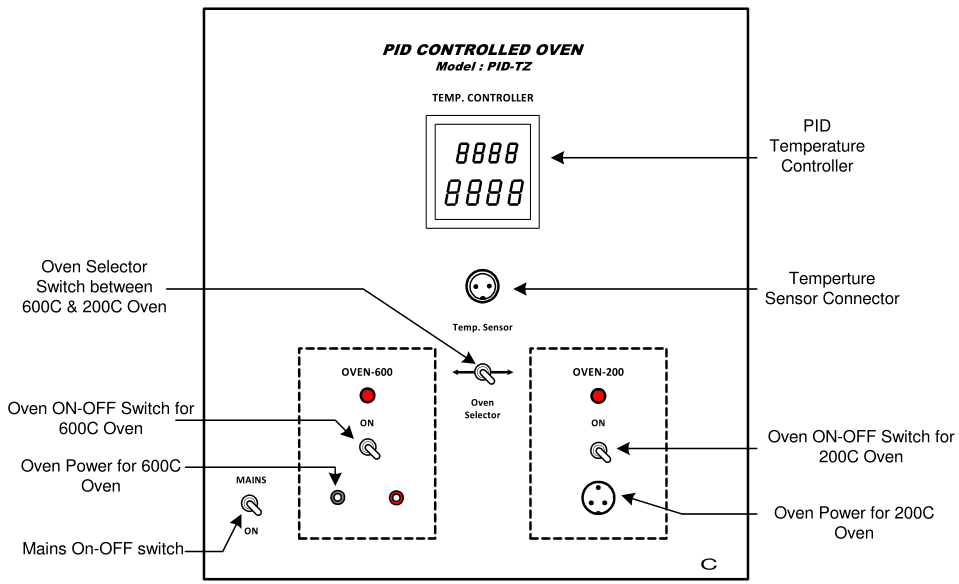
\includegraphics[scale = 0.8]{Figures/PID-TZ.png}
    \caption{PID Controlled Oven, PID-TZ}
    \label{fig:pid-tz}
\end{figure*}
\subsection{Constant Current Source, Model : CCS-01}
It is an IC regulated current generator to provide a constant current to the
outer probes irrespective of the changing resistance of the sample due to change in
temperatures. The basic scheme is to use the feedback principle to limit the load
current of the supply to preset maximum value. Variations in the current are
achieved by a potentiometer included for that purpose. The supply is a highly
regulated and practically ripples free $DC$ source. The constant current source is
suitable for the resistivity measurement of thin films of metals/ alloys and
semiconductors like germanium.
\begin{figure*}
    \centering
    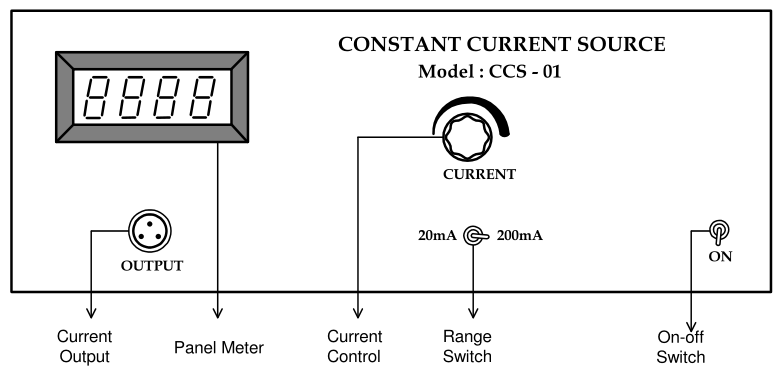
\includegraphics[scale = 0.8]{Figures/ccs-01.png}
    \caption{Constant Current Source, CCS-01}
    \label{fig:ccs-01}
\end{figure*}

\subsection{Low Current Source, Model : LCS-02}
Low Constant Current Sources are needed when the sample resistance, either
inherently or due to contact resistances, is large. These include the resistivity
measurement of silicon wafers or high resistivity film deposits.

\begin{figure*}
    \centering
    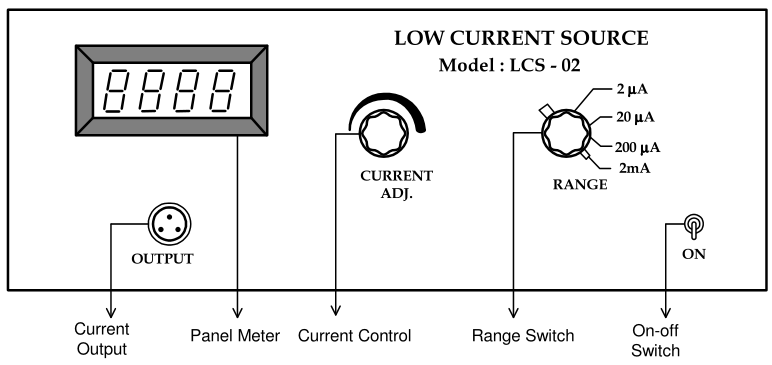
\includegraphics[scale = 0.8]{Figures/lcs-02.png}
    \caption{Low Current Source, LCS-02}
    \label{fig:lcs-02}
\end{figure*}

\subsection{DC Microvoltmeter, Model DMV-001}
Digital Microvoltmeter, DMV-001 is a very versatile multipurpose instrument
for the measurement of low $DC$ voltage. It has 5 decade ranges from $\SI{1}{\milli \volt}$ to $\SI{10}{\volt}$ with
100\% over-ranging. This instrument uses a very well designed chopper stabilized IC amplifier.
This amplifier offers exceptionally low offset voltage and input bias parameters,
combined with excellent speed characteristics.
\begin{figure*}
    \centering
    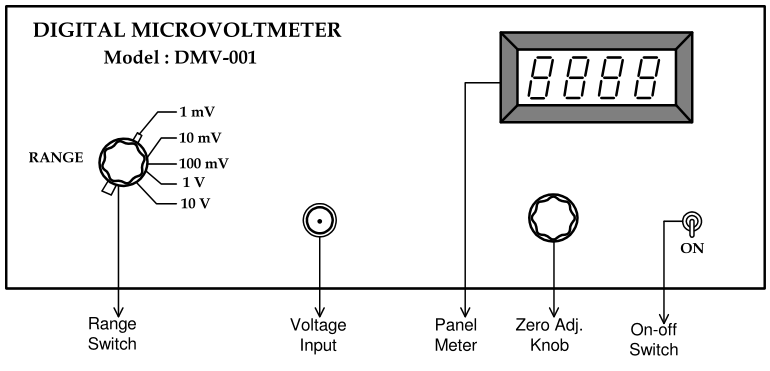
\includegraphics[scale = 0.8]{Figures/dmv-001.png}
    \caption{Digitral Microvoltmeter, DMV-001}
    \label{fig:dmv}
\end{figure*}
\subsection{Four Probes Arrangement}
It has four individually spring loaded probes. The probes are collinear and
equally spaced. The probes are mounted in a teflon bush, which ensure a good
electrical insulation between the probes. A teflon spacer near the tips is also provided
to keep the probes at equal distance. The probe arrangement is mounted in a suitable
stand, which also holds the sample plate and RTD sensor. This stand also serves as
the lid of PID Controlled Oven. Proper leads are provided for current, Voltage and
Temp. measurement with their universal connectors. For current measurement there is
three pin connector which can be connected to the CCS-01/ LCS-02 as per
requirement of sample. For voltage measurement BNC connector is used connected to
DMV-001 unit. For temperature measurement, a two pin connector is provided for
connection with PID- Controlled oven unit PID-200 at connector marked as
Temperature Sensor. Three levelling screws are provided in Four Probe arrangement by which we can adjust the
level of plateform to make it horizontal. A probe holding screw is provided at the collar of the
arrangement. Initially it should be in loose position, to allow free movement of Probe Pipe.
After placing the sample the Probe Pipe should be lowered so that all four pins touches the
sample. The pipe is further pressed very lightly so that the assured firm contact is made of all Four
Pins with the sample. The probe holding screw is tightened at this position making the arrangement ready to use.
\begin{figure}
    \centering
    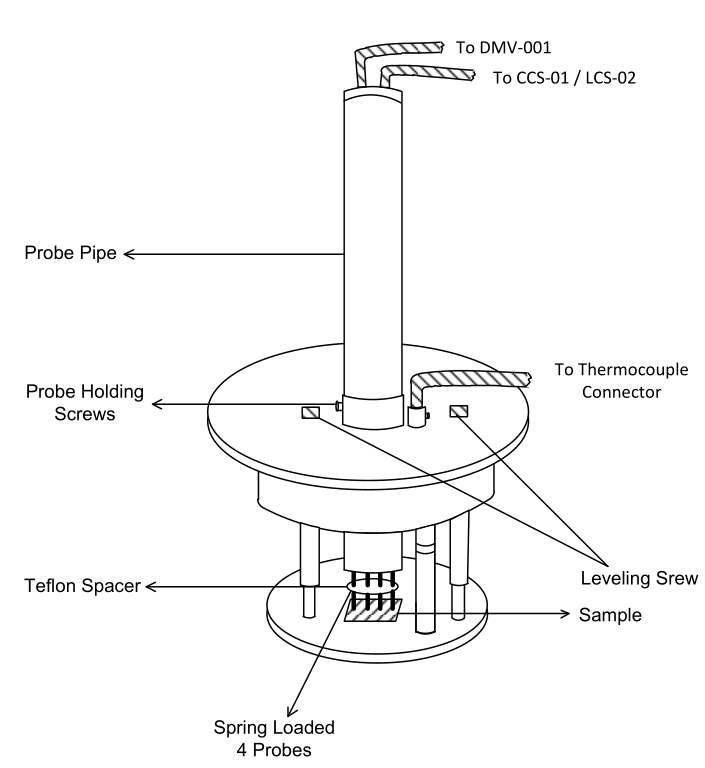
\includegraphics[scale = 0.56]{Figures/four-probe-arrangement.png}
    \caption{Four Probe Arrangement}
    \label{fig:4-probe}
\end{figure}


\section{Theory}
Four sharp probes are placed on a flat surface of the material to be measured (figure (\ref{fig:model})).
The current is passed through the two outer electrodes, and the floating potential is measured
across the inner pair. If the flat surface on which the probes rest is adequately large, it may be
considered to be a semi-infinite volume. To prevent minority carrier injection and make good
contacts, the surface on which the probes rest, maybe mechanically lapped.

\par
The experimental circuit used for measurement is illustrated schematically in figure (\ref{fig:circuit}).
A nominal value of probe spacing, which has been found satisfactory, is an equal distance of $\SI{2.00}{\milli \metre}$ between adjacent probes.

\par

In order to use four-probe, we assume: the resistivity of the material is uniform in the area of measurement, if there is minority carrier injection into the semiconductor by the current - carrying
electrodes, most of the carriers recombine near the electrodes so that their effect on the
conductivity is negligible. (This means that the measurements should be made on surface,
which has a high recombination rate, such as mechanical by lapped surfaces), the surface on which the probes rest is flat with no surface leakage, the four probes used for resistivity measurements are equally spaced and collinear, the diameter of the contact between the metallic probes and the semiconductor should be small compared to the distance between probes, the surfaces of the material may be either conducting or non-conducting.

\begin{figure}
    \centering
    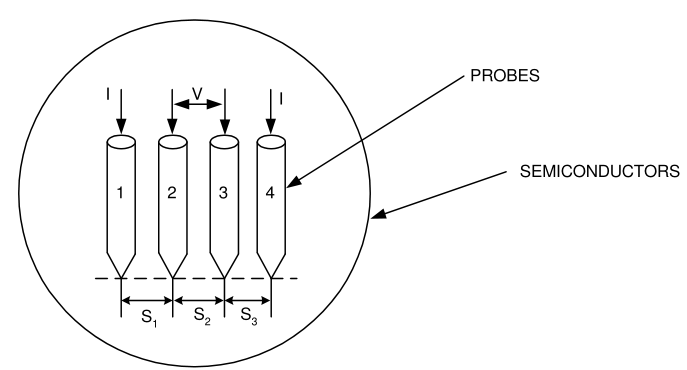
\includegraphics[scale = 0.57]{Figures/model-for-resistivity.png}
    \caption{Model for the four probe resistivity measurement}
    \label{fig:model}
\end{figure}

\begin{figure}
    \centering
    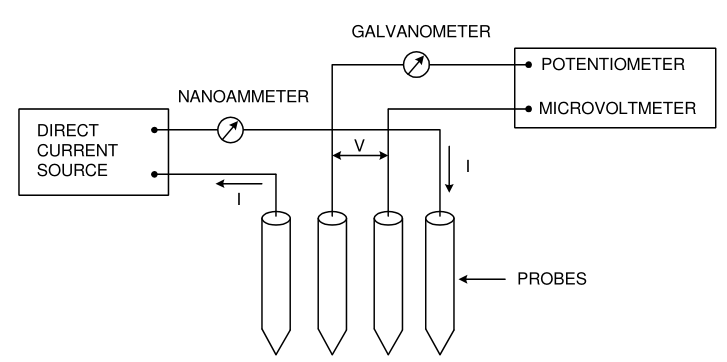
\includegraphics[scale = 0.55]{Figures/circuit-for-resistivity.png}
    \caption{Circuit used for resistivity measurement}
    \label{fig:circuit}
\end{figure}

\subsection{Resistivity measurements on a large sample}
One added boundary condition is required to treat this case namely, the probes are far
from any of the other surfaces of the sample and the sample can thus be considered a semi-
infinite volume of uniform resistivity material. Figure (\ref{fig:model}) shows the geometry of this case.

\par
The floating potential $V_f$ a distance $r$ from an electrode carrying a current $I$ in a
material of resistivity $\rho_0$ is given by
\begin{equation}
    V_f = \dfrac{\rho_0 I}{2 \pi r}
\end{equation}
From here, after some manipulations, we can calculate the resistivity (for the case in figure (\ref{fig:model})) as:
\begin{equation}
    \rho_0 = \dfrac{V}{I} - \dfrac{2 \pi}{\Bigg( \dfrac{1}{S_1} + \dfrac{1}{S_3} - \dfrac{1}{S_1 + S_2} - \dfrac{1}{S_2 + S_3} \Bigg)} 
\end{equation}
When the point spacings are equal, that is, $S_1 = S_2 = S_3 = S$ the above simplifies to:
\begin{equation}
    \rho_0 = \dfrac{V}{I} 2 \pi S
\end{equation}
\subsection{Resistivity measurements on a thin slice-conducting bottom surface}
Two boundary conditions must be met in this case; the top surface of the slice must be
a reflecting (non-conducting) surface and the bottom surface must be an absorbing
(conducting) surface. Since the two boundaries are parallel, a solution by the method of
images requires for each current source an infinite series of images along a line normal to the
plane and passing through the current source.

\par
The model for this case is shown in figure (\ref{fig:images}). The side surface of the slice is assumed to
be far from the area of measurement and, therefore, only the effect of the bottom surface
needs to be considered. In this analysis equal probe spacing $S$ shall be assumed. The width of
the slice is $W$. The array of images needed is indicated in figure (\ref{fig:images}). where the polarity and
spacing of the first few images are as shown.
\par
For this case, the resistivity is given by
\begin{equation}
    \rho = \dfrac{\rho}{G_6 (W/S)}
\end{equation}
where $G_6(W/S)$ is a correction term given by
\begin{equation}
\resizebox{0.4\textwidth}{!}{$G_6 (\frac{W}{S}) = 1 + 4 \frac{S}{W} \sum(-1)^{n}
        \Bigg[ \frac{1}{\sqrt{\big(\frac{S}{W} \big)^2 + (2n)^2}} - \frac{1}{\sqrt{\big(2 \frac{S}{W} \big)^2 + (2n)^2}}\Bigg]$}
\end{equation}

\begin{figure}
    \centering
    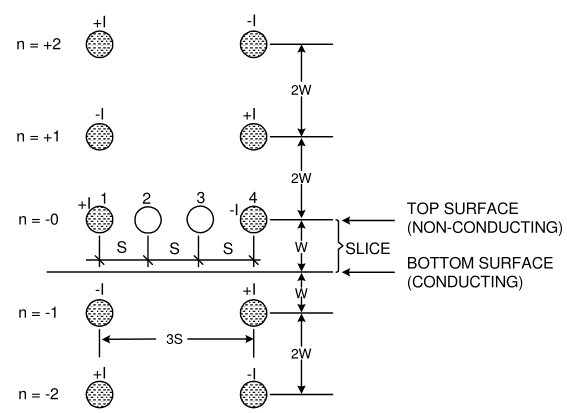
\includegraphics[scale = 0.7]{Figures/images.png}
    \caption{The resistivity probes on a slice with conducting bottom
surface}
    \label{fig:images}
\end{figure}
\subsection{Resistivity measurements on a thin slice-non-conducting bottom surface}
The model for these measurements is like the case 2, except that the bottom surface of
the slice is nonconducting. This means that all the images of  have the same charge as
the current source. Then, in this case,
\begin{equation}
    \rho = \dfrac{\rho}{G_7 (W/S)}
\end{equation}
where
\begin{equation}
    \resizebox{0.4\textwidth}{!}{$G_7 (\frac{W}{S}) = 1 + 4 \frac{S}{W} \sum
        \Bigg[ \frac{1}{\sqrt{\big(\frac{S}{W} \big)^2 + (n)^2}} - \frac{1}{\sqrt{\big(2 \frac{S}{W} \big)^2 + (2n)^2}}\Bigg]$}
\end{equation}
For smaller
values of $W/S$, the function $G_7 (W/S)$ approaches the case for an infinitely thin slice, or
\begin{equation}
\label{g7ws}
    G_7 (W/S) = \dfrac{2S}{W} \ln 2
\end{equation}
\begin{figure*}
    \centering
    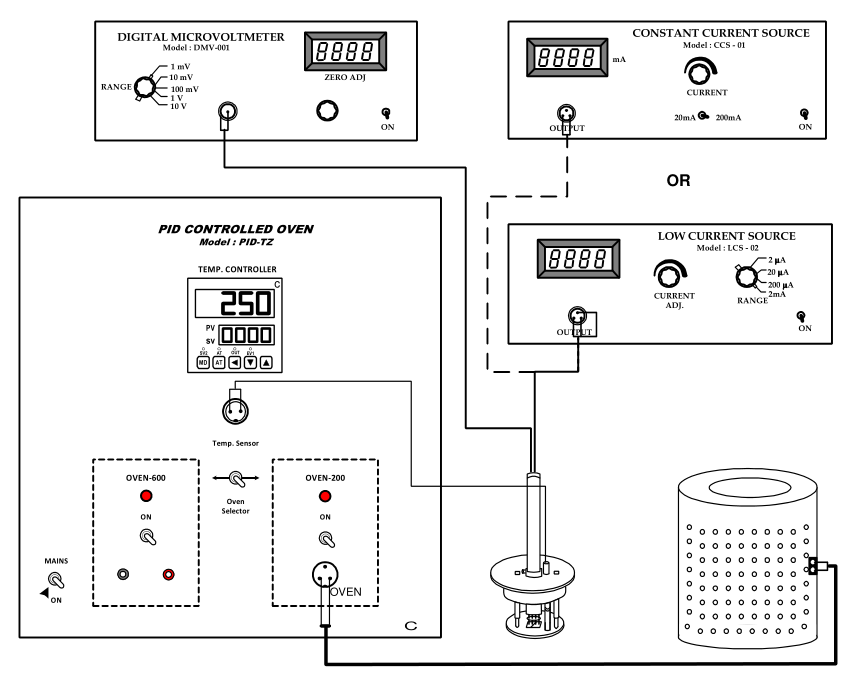
\includegraphics[scale = 0.8]{Figures/connection-diagram.png}
    \caption{Connection diagram for the set up}
    \label{fig:connector}
\end{figure*}
\begin{figure}
    \centering
    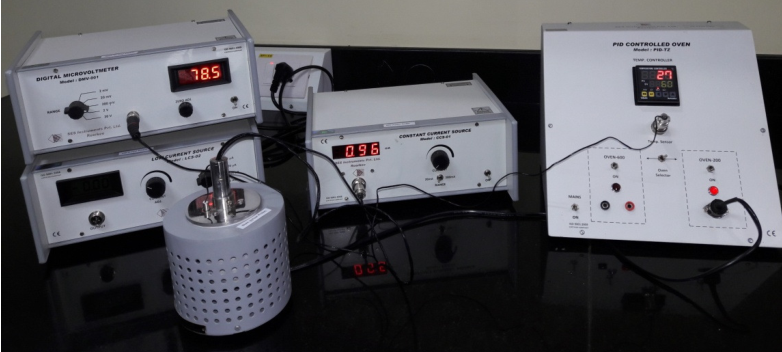
\includegraphics[scale = 0.5]{Figures/experimental-setup.png}
    \caption{Complete experimental set up for the four-probe part}
    \label{fig:set-up}
\end{figure}
\subsection{Direct and Indirect band-gaps in semiconductors}
The band gap represents the minimum energy difference between the top of the valence band and
the bottom of the conduction band, However, the top of the valence band and the bottom of the
conduction band are not generally at the same value of the electron momentum ($k$). In a direct
band gap semiconductor, the top of the valence band and the bottom of the conduction band
occur at the same value of momentum ($k$). In an indirect band gap semiconductor, the maximum energy of the valence band occurs at a
different value of momentum to the minimum in the conduction band energy. 

\par
The difference between the two is most important in optical devices. Each photon of energy $E$
has momentum $p = E / c$, where $c$ is the velocity of light. An optical photon has an energy of the order of $\SI{1e-19}{\joule}$, and, since $c = \SI{3e8}{\metre \per \second}$, a typical photon has a very small amount of
momentum.

\par

A photon of energy $E_g$, where $E_g$ is the band gap energy, can produce an electron-hole pair in a
direct band gap semiconductor quite easily, because the electron does not need to be given very
much momentum. However, an electron must also undergo a significant change in its momentum
for a photon of energy $E_g$ to produce an electron-hole pair in an indirect band gap semiconductor.
This is possible, but it requires such an electron to interact not only with the photon to gain energy,
but also with a lattice vibration called a phonon in order to either gain or lose momentum.

\par
The indirect process proceeds at a much slower rate, as it requires three entities to intersect in order
to proceed: an electron, a photon and a phonon. The same principle applies to recombination of
electrons and holes to produce photons. The recombination process is much more efficient for a
direct band gap semiconductor than for an indirect band gap semiconductor, where the process
must be mediated by a phonon.

\par
As a result of such considerations, gallium arsenide and other direct band gap semiconductors are
used to make optical devices such as LEDs and semiconductor lasers, whereas silicon, which is an
indirect band gap semiconductor, is not. The table in the next section lists a number of different
semiconducting compounds and their band gaps, and it also specifies whether their band gaps are
direct or indirect.

\begin{figure}
    \centering
    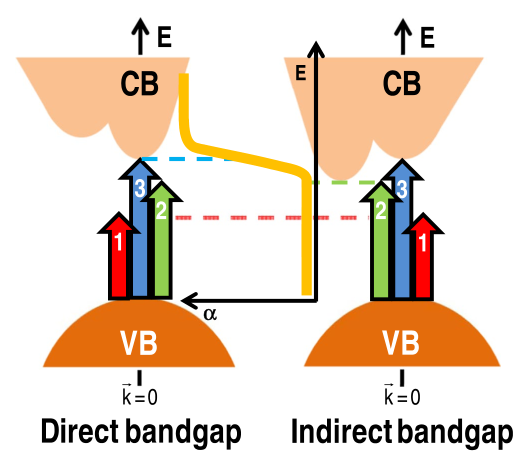
\includegraphics[scale = 0.6]{Figures/simplified-energy-diagram.png}
    \caption{Simplified energy diagram illustrating the valence (VB) and conduction (CB) bands of direct and
indirect band-gap semiconductors.}
    \label{fig:bandgaps}
\end{figure}

A common and simple method for determining whether a band gap is direct or indirect uses absorption spectroscopy. By plotting certain powers of the absorption coefficient against photon energy, one can normally tell both what value the band gap is, and whether or not it is direct.
\par
For a direct band gap, the absorption coefficient $\alpha$ is related to light frequency according to the following formula:
\begin{equation}
    \alpha = B (h \nu - E_g)^{1/2}
\end{equation}
for direct gap semiconductor and
\begin{equation}
    \alpha = B (h \nu - E_g)^2
\end{equation}
for an indirect gap semiconductor (assuming photon energy is very very less than band gap energy) and $B$ being a constant.
\section{Observations}
The current versus voltage readings for n-Al is given in table (\ref{tab:altable}) and is plotted in figure (\ref{fig:alplot}). The current versus voltage readings for n-Si is given in table (\ref{tab:sitable}) and is plotted in figure (\ref{fig:siplot}). The current versus voltage readings for n-Ge is given in table (\ref{tab:getable}) and is plotted in figure (\ref{fig:geplot}). The temperature versus voltage readings for Ge wafer at constant current is given in table (\ref{tab:temptable}). The plot between $\ln \rho \sim 1/T$ is plotted in figure (\ref{fig:tempplot}). The plot between energy and absorption coefficient to the second power for ZnO is given in figure (\ref{:znoplot}) for direct band gap. The plot between energy and the square root of absorption coefficient for polymer is given in figure (\ref{:polymerplot}) for indirect band gap. The following additional observations were made:
\begin{enumerate}
    \item No. of commercial Al foils: 16
    \item Thickness of one foil: \SI{0.001}{\centi \metre}
    \item Thickness of Al Stack: \SI[separate-uncertainty=true]{0.16 \pm 0.01}{\milli \metre}
    \item Probe distance ($S$): $0.200 \pm 2\%$ cm (fixed)
    \item Thickness for n-Si: $0.50 \pm 2\%$ mm
    \item Thickness for Ge wafer: $0.50 \pm 2\%$ mm
    \item Probe current for Ge wafer: $\SI{5}{\milli \ampere}$ (fixed).
    \item Thickness of ZnO: $\SI{1}{\micro \metre}$
    \item Thickness of polymer: $\SI{150}{\nano \metre}$
\end{enumerate}
\begin{table}[]
\caption{Readings for calculation of resistivity of Aluminium}
\label{tab:altable}
\begin{tabular}{@{}cc@{}}
\toprule
\textbf{I (mA)} & \textbf{V (mV)} \\ \midrule
0               & 0               \\
20              & 0.004           \\
39.5            & 0.01            \\
59.7            & 0.016           \\
80.2            & 0.023           \\
100             & 0.029           \\
120             & 0.036           \\
140             & 0.042           \\
160             & 0.049           \\
180             & 0.054           \\
199.4           & 0.061           \\ \bottomrule
\end{tabular}
\end{table}


% Please add the following required packages to your document preamble:
% \usepackage{booktabs}
\begin{table}[]
\caption{Readings for calculation of resistivity of Silicon}
\label{tab:sitable}
\begin{tabular}{@{}cc@{}}
\toprule
\textbf{I (mA)} & \textbf{V (mV)} \\ \midrule
0               & 0               \\
0.001           & 0.221           \\
0.002           & 0.313           \\
0.003           & 0.37            \\
0.004           & 0.466           \\
0.005           & 0.616           \\
0.01            & 1.134           \\
0.02            & 2.16            \\
0.03            & 3.21            \\
0.04            & 4.23            \\
0.05            & 5.34            \\
0.06            & 6.4             \\
0.08            & 8.4             \\
0.1             & 10.55           \\
0.2             & 21              \\
0.3             & 31.4            \\
0.402           & 42              \\
0.501           & 52.4            \\
0.601           & 63              \\
0.67            & 69.5            \\ \bottomrule
\end{tabular}
\end{table}

% Please add the following required packages to your document preamble:
% \usepackage{booktabs}
\begin{table}[]
\caption{Readings for calculation of resistivity of  Germanium}
\label{tab:getable}
\begin{tabular}{@{}cc@{}}
\toprule
\textbf{I (mA)} & \textbf{V (mV)} \\ \midrule
0.16            & 12              \\
0.56            & 43              \\
0.68            & 53              \\
0.74            & 57              \\
0.86            & 66              \\
0.95            & 73              \\
1.11            & 85              \\
1.28            & 99              \\
1.38            & 107             \\
1.45            & 112             \\
1.63            & 125             \\
1.78            & 138             \\
1.86            & 144             \\
1.98            & 155             \\
2.15            & 167             \\
2.29            & 178             \\
2.57            & 200             \\
2.73            & 212             \\
2.87            & 223             \\
3.12            & 243             \\
3.32            & 259             \\
3.48            & 272             \\
3.83            & 298             \\
4.09            & 319             \\
4.24            & 331             \\
4.58            & 357             \\
4.74            & 370             \\
5.01            & 391             \\
5.38            & 420             \\
5.57            & 435             \\ \bottomrule
\end{tabular}
\end{table}

% Please add the following required packages to your document preamble:
% \usepackage{booktabs}
\begin{table}[]
\caption{Variation of resistivity of Germanium wafer with temperature at constant current $\SI{5}{\milli \ampere}$}
\label{tab:temptable}
\begin{tabular}{@{}cccc@{}}
\toprule
\textbf{T ($\degree C$)} & \textbf{V (mV)} & \textbf{1/T ($10^{-3} K^{-1}$)} & \textbf{$\ln \rho$} \\ \midrule
80             & 0.14              & 2.832             & -1.200                \\
90             & 0.102             & 2.754             & -1.337                \\
100            & 0.079             & 2.680             & -1.448                \\
110            & 0.061             & 2.610             & -1.561                \\
120            & 0.045             & 2.544             & -1.693                \\
130            & 0.035             & 2.480             & -1.802                \\
140            & 0.028             & 2.420             & -1.899                \\
150            & 0.022             & 2.363             & -2.003                \\
160            & 0.017             & 2.309             & -2.115                \\
170            & 0.014             & 2.257             & -2.200                \\
180            & 0.011             & 2.207             & -2.304                \\ \bottomrule
\end{tabular}
\end{table}
\begin{figure}
    \centering
    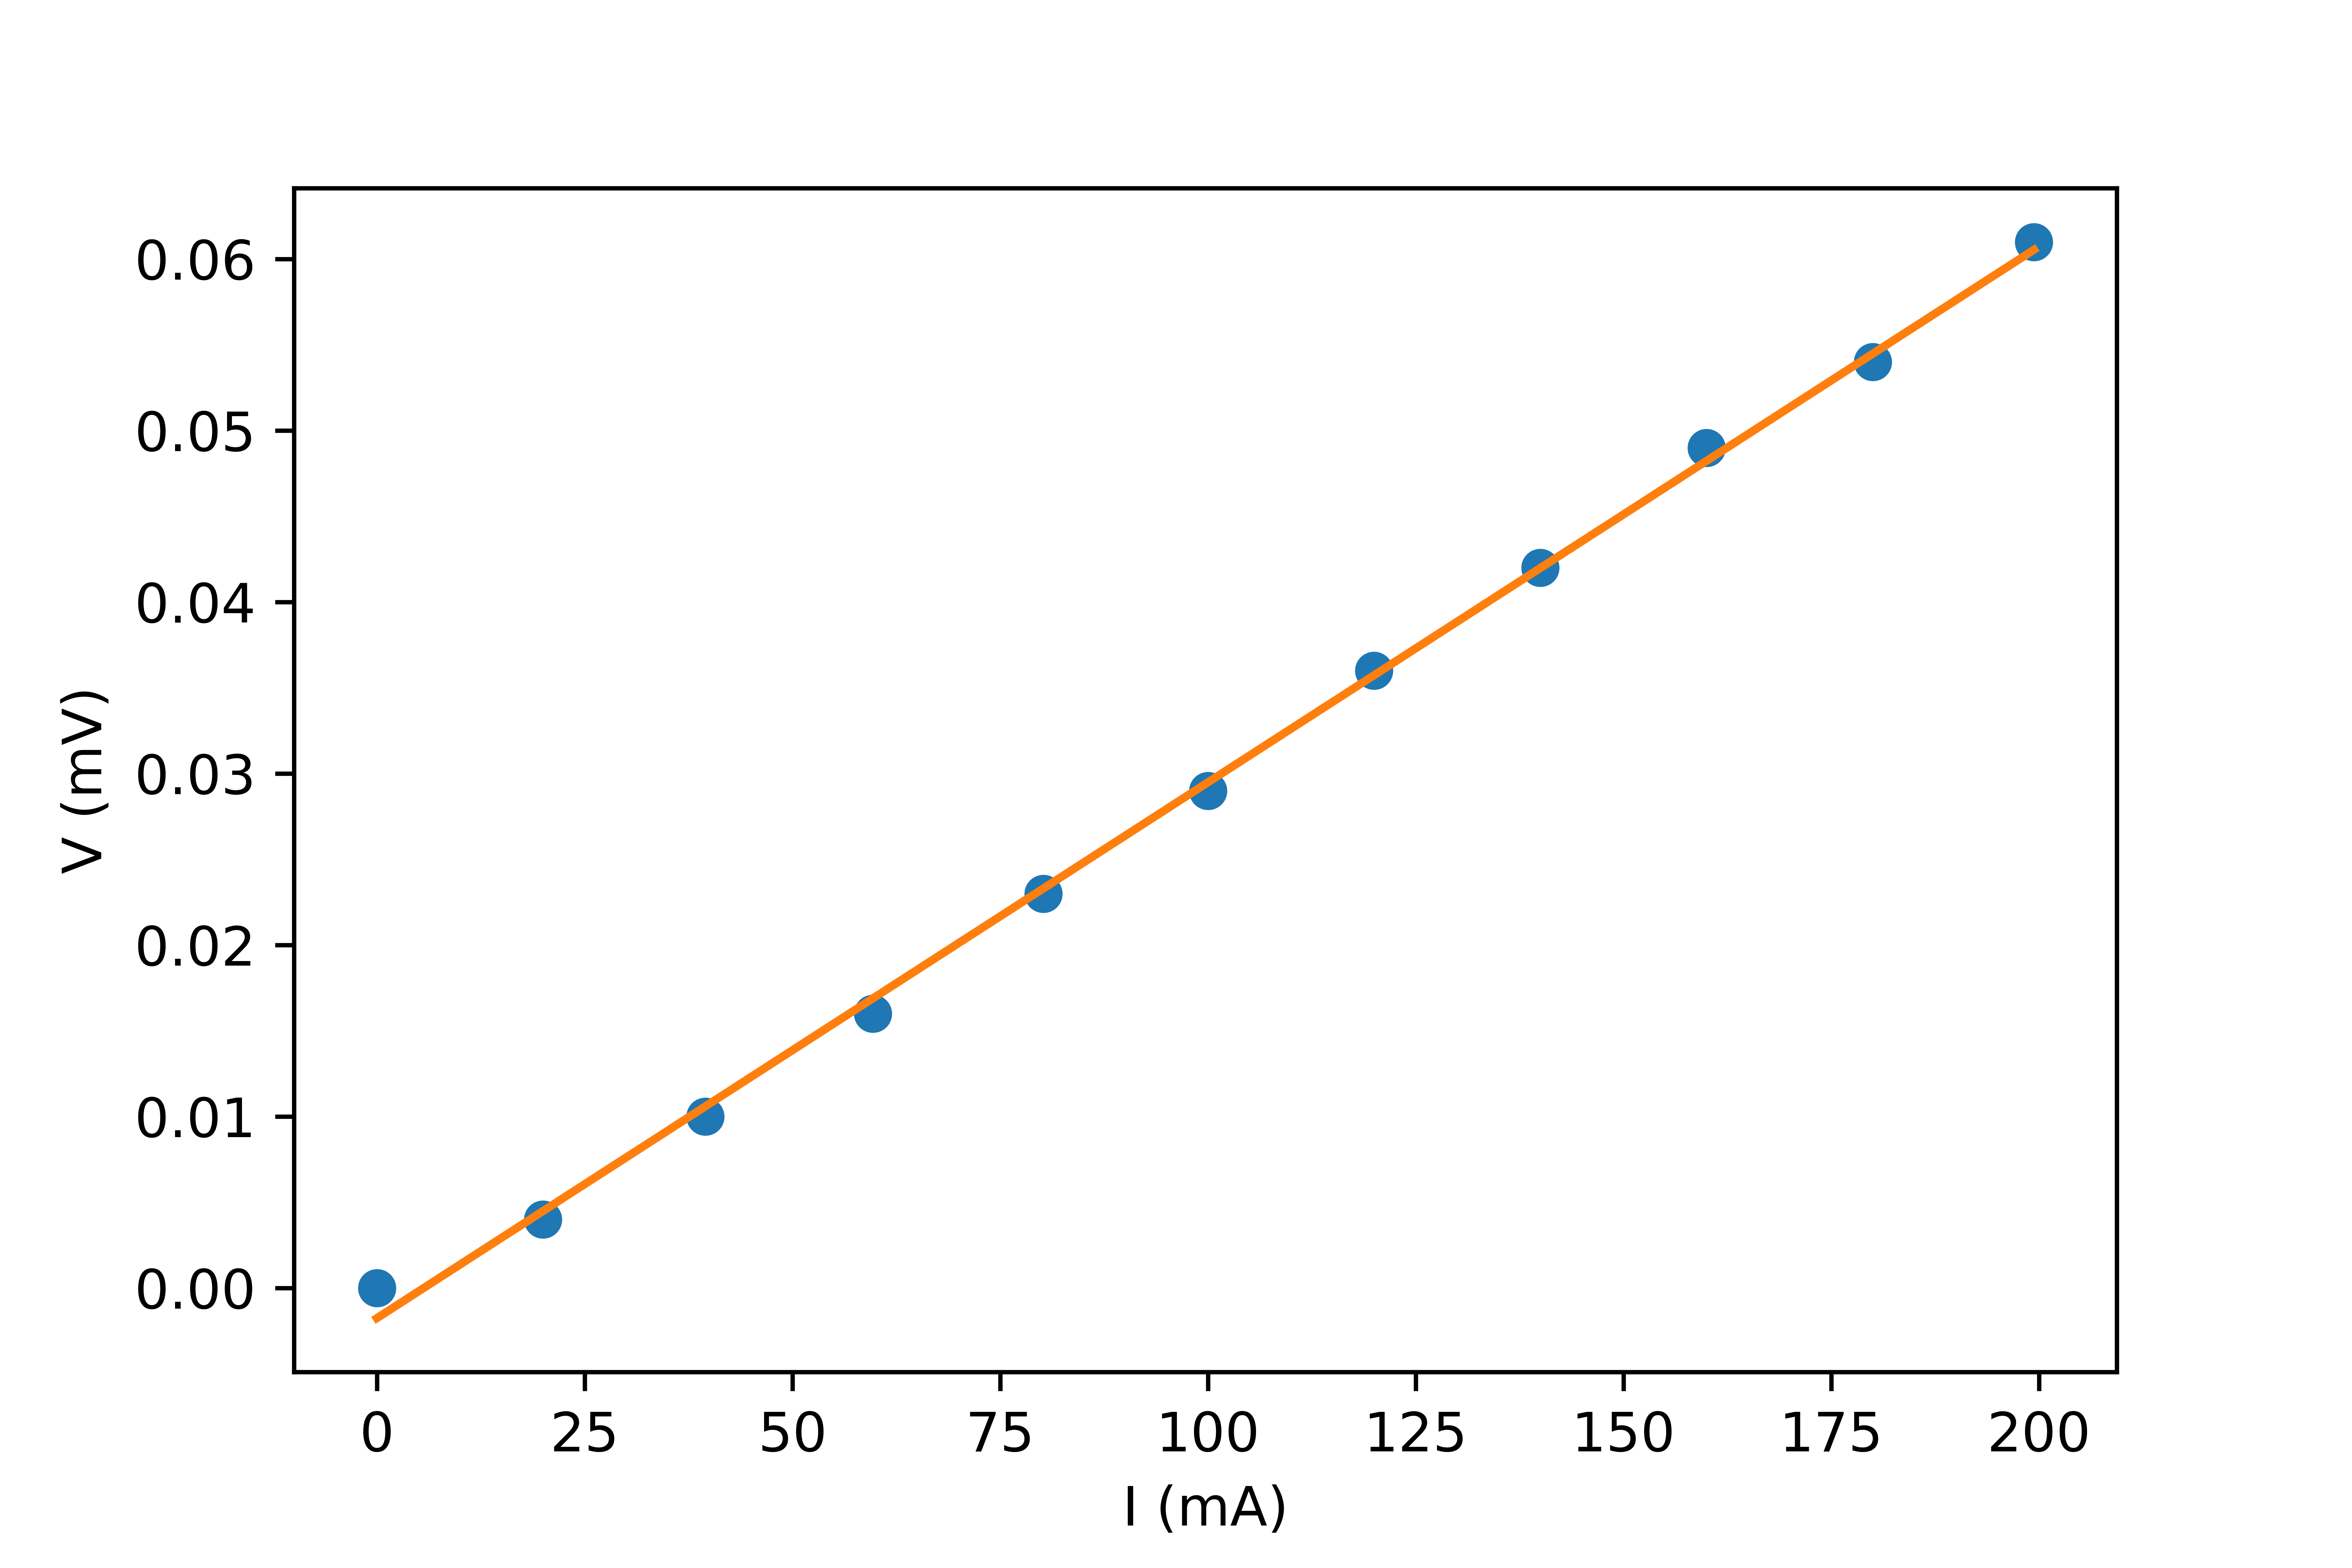
\includegraphics[scale = 0.56]{Figures/plot-n-Al.png}
    \caption{The $V \sim I$ plot for n-Al}
    \label{fig:alplot}
\end{figure}
\begin{figure}
    \centering
    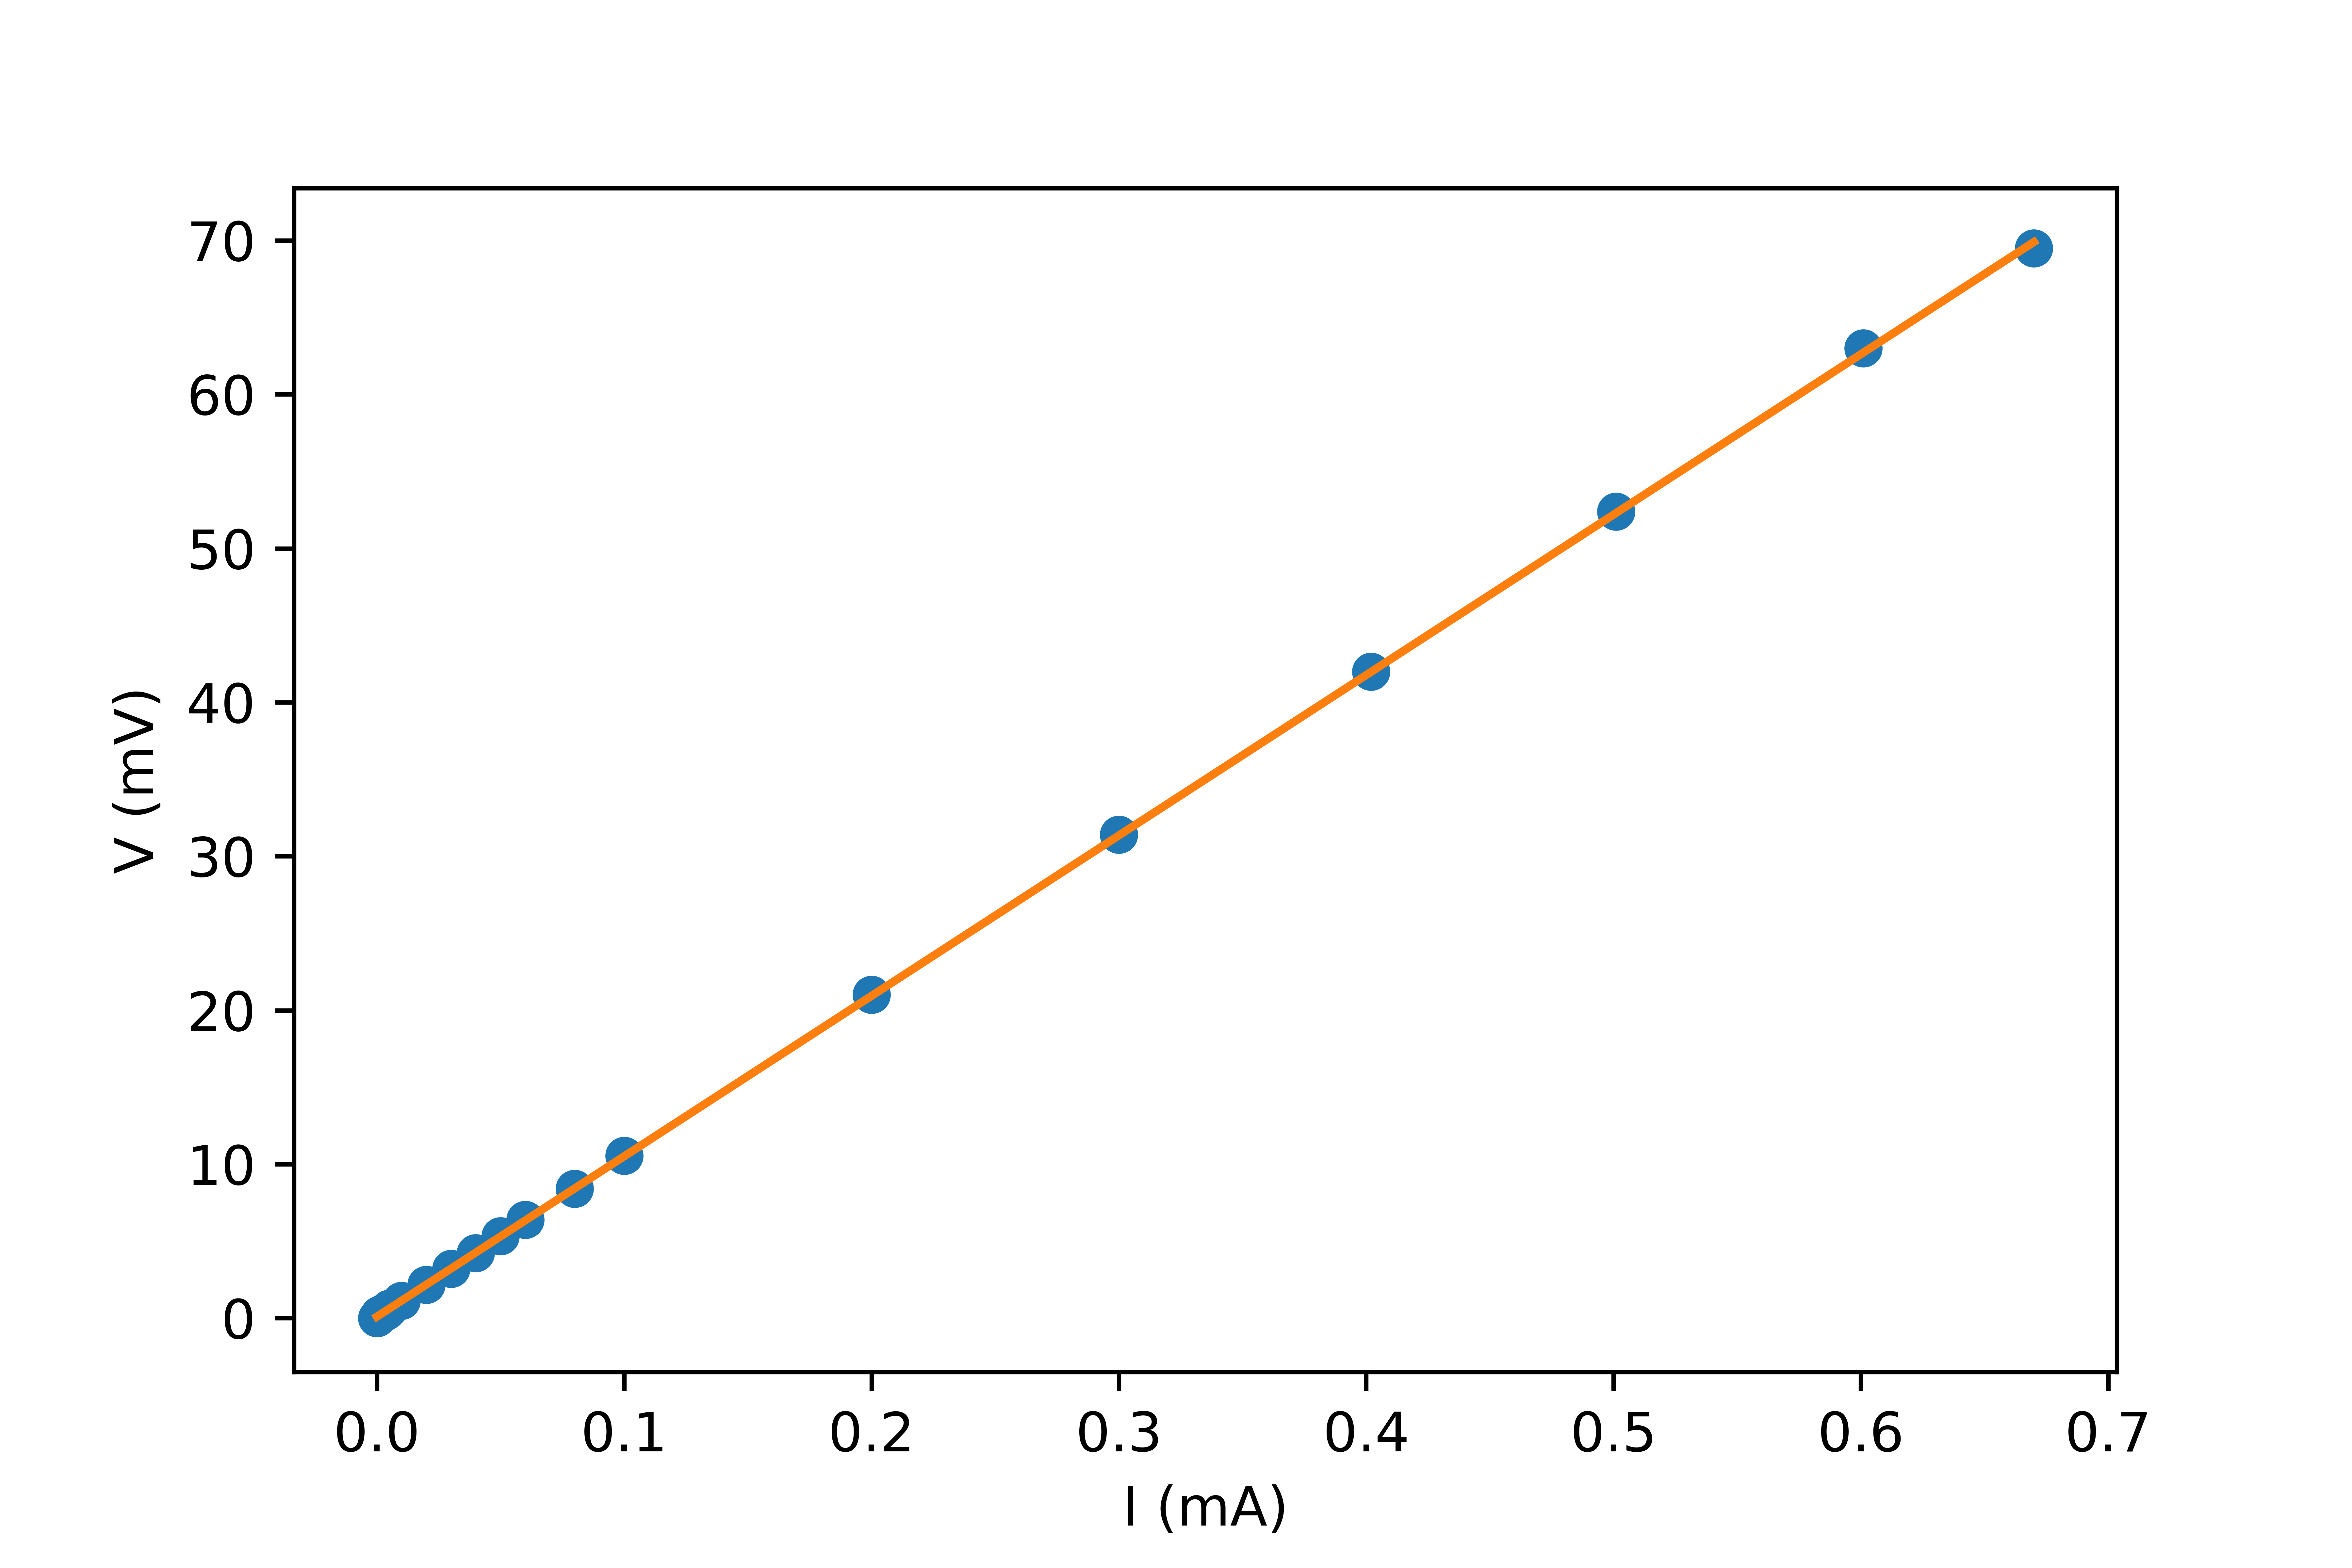
\includegraphics[scale = 0.56]{Figures/plot-n-Si.png}
    \caption{The $V \sim I$ plot for n-Si}
    \label{fig:siplot}
\end{figure}
\begin{figure}
    \centering
    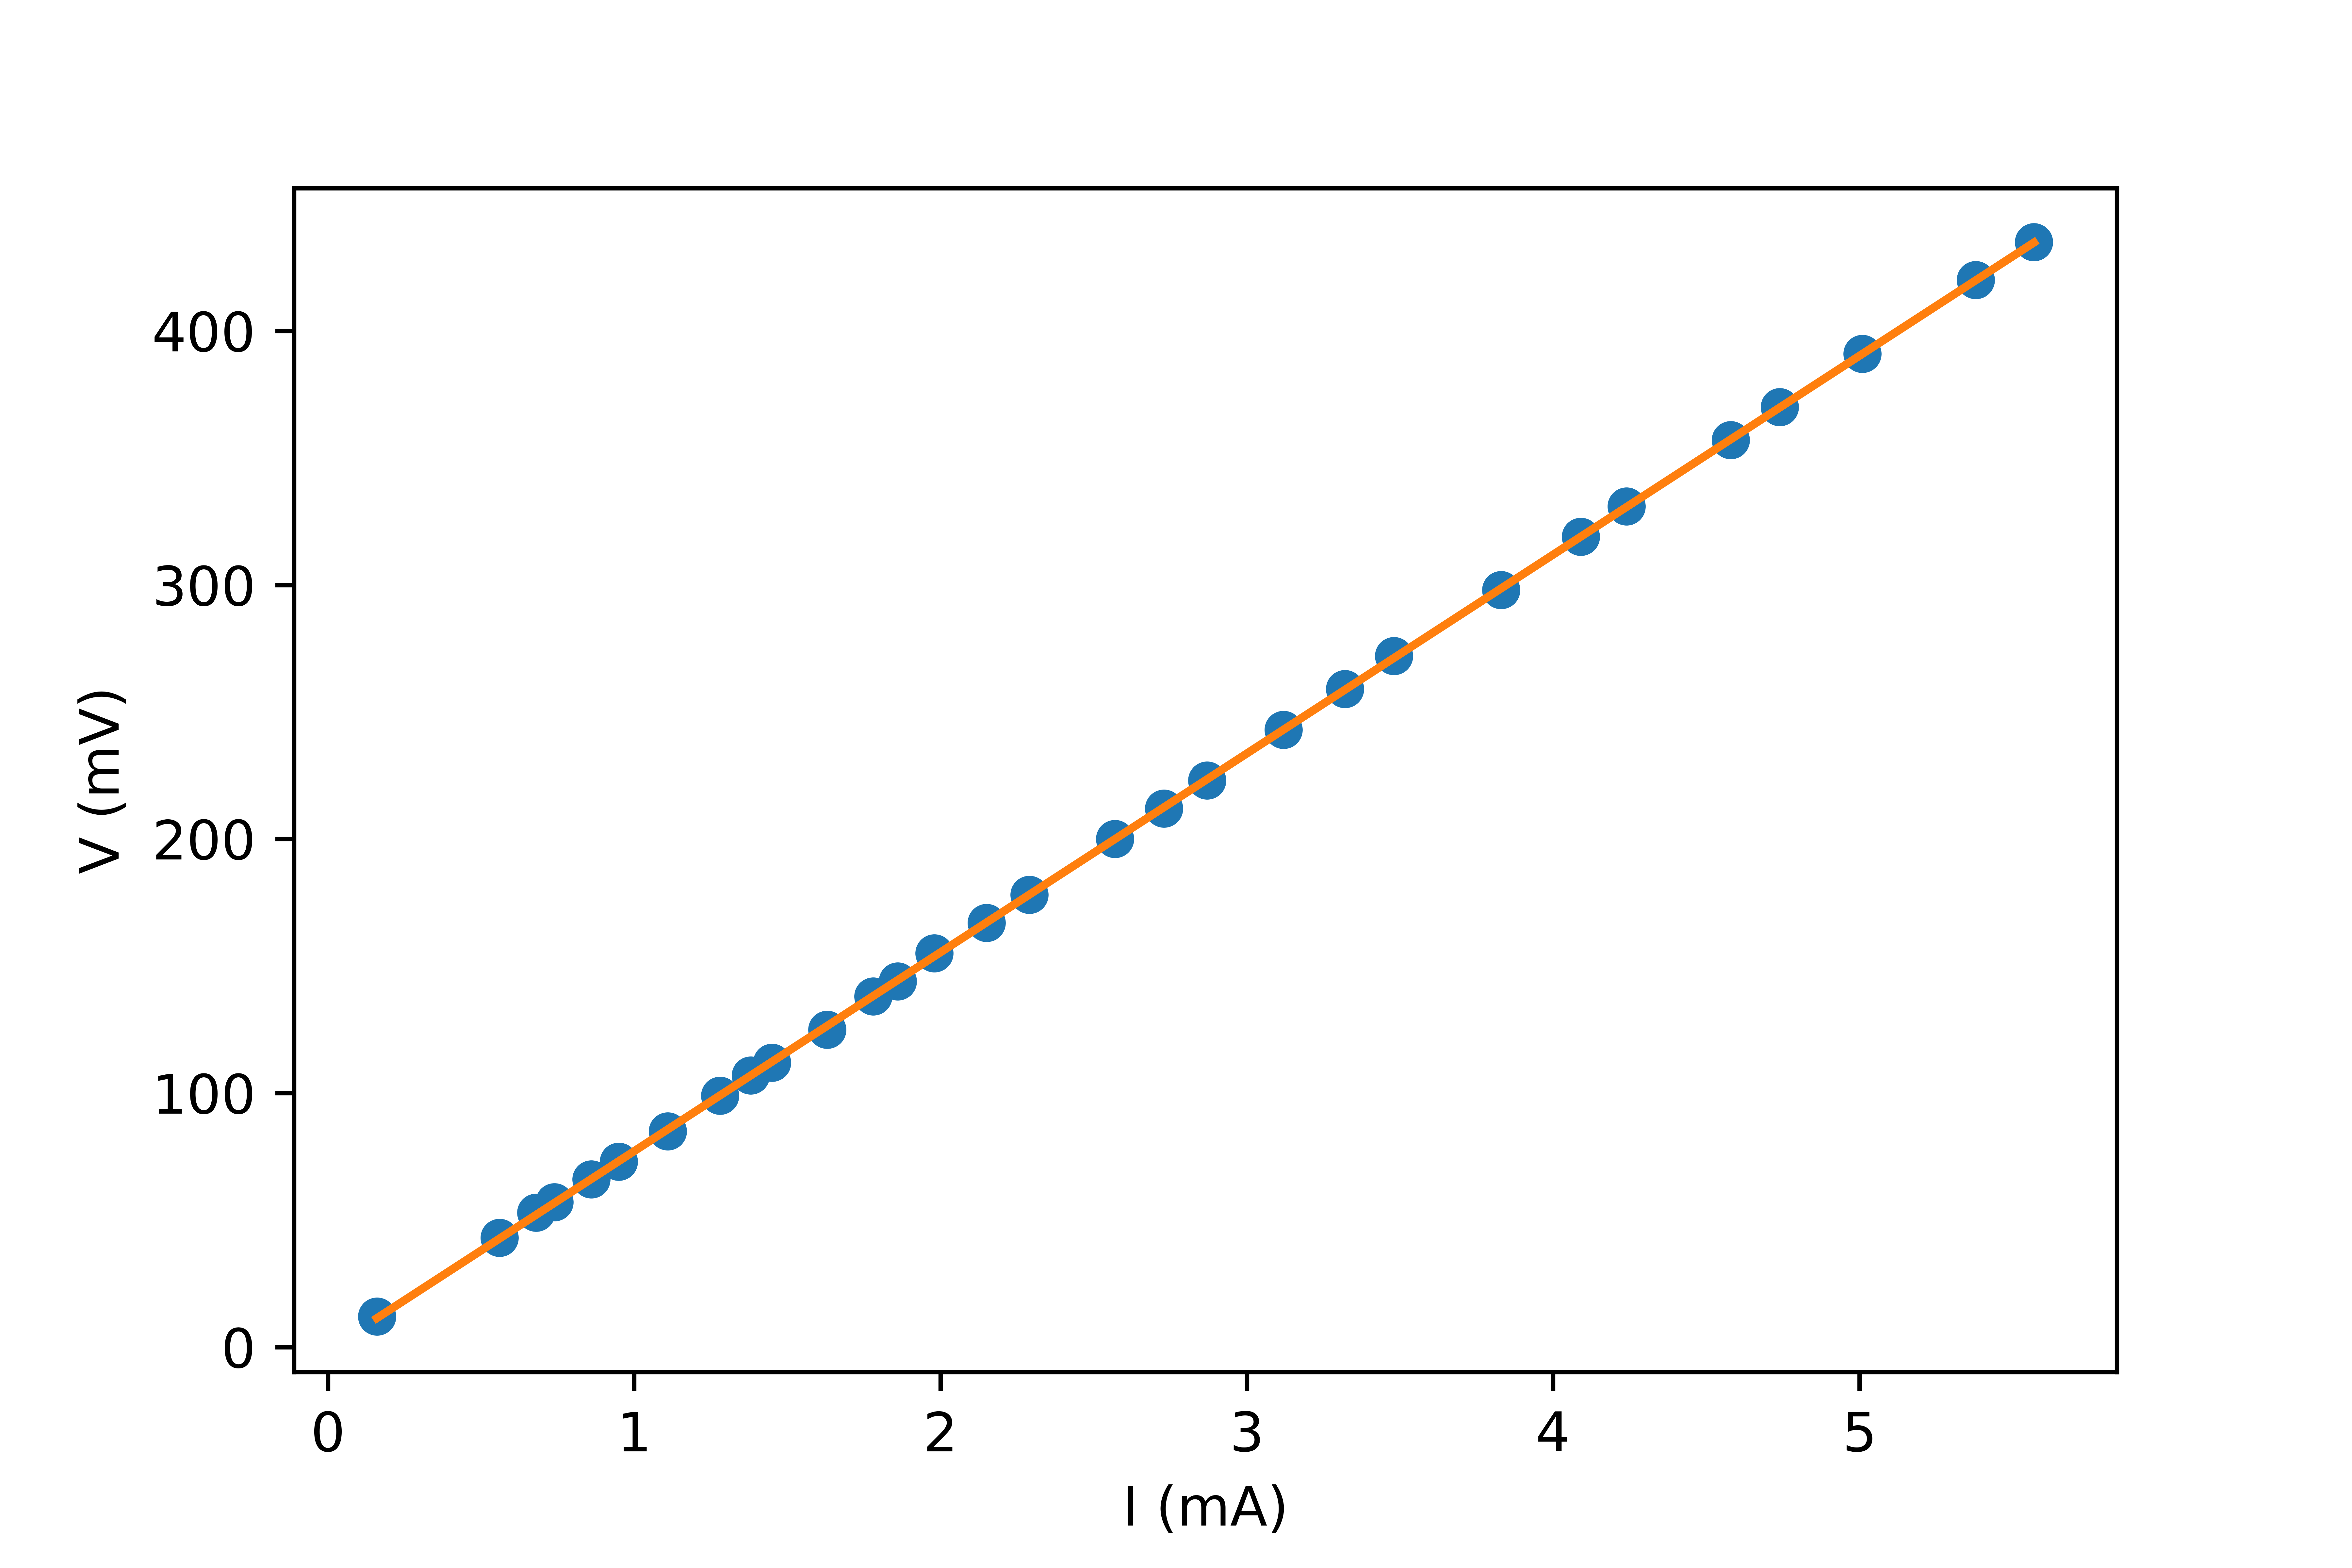
\includegraphics[scale = 0.56]{Figures/plot-n-Ge.png}
    \caption{The $V \sim I$ plot for n-Ge}
    \label{fig:geplot}
\end{figure}
\begin{figure}
    \centering
    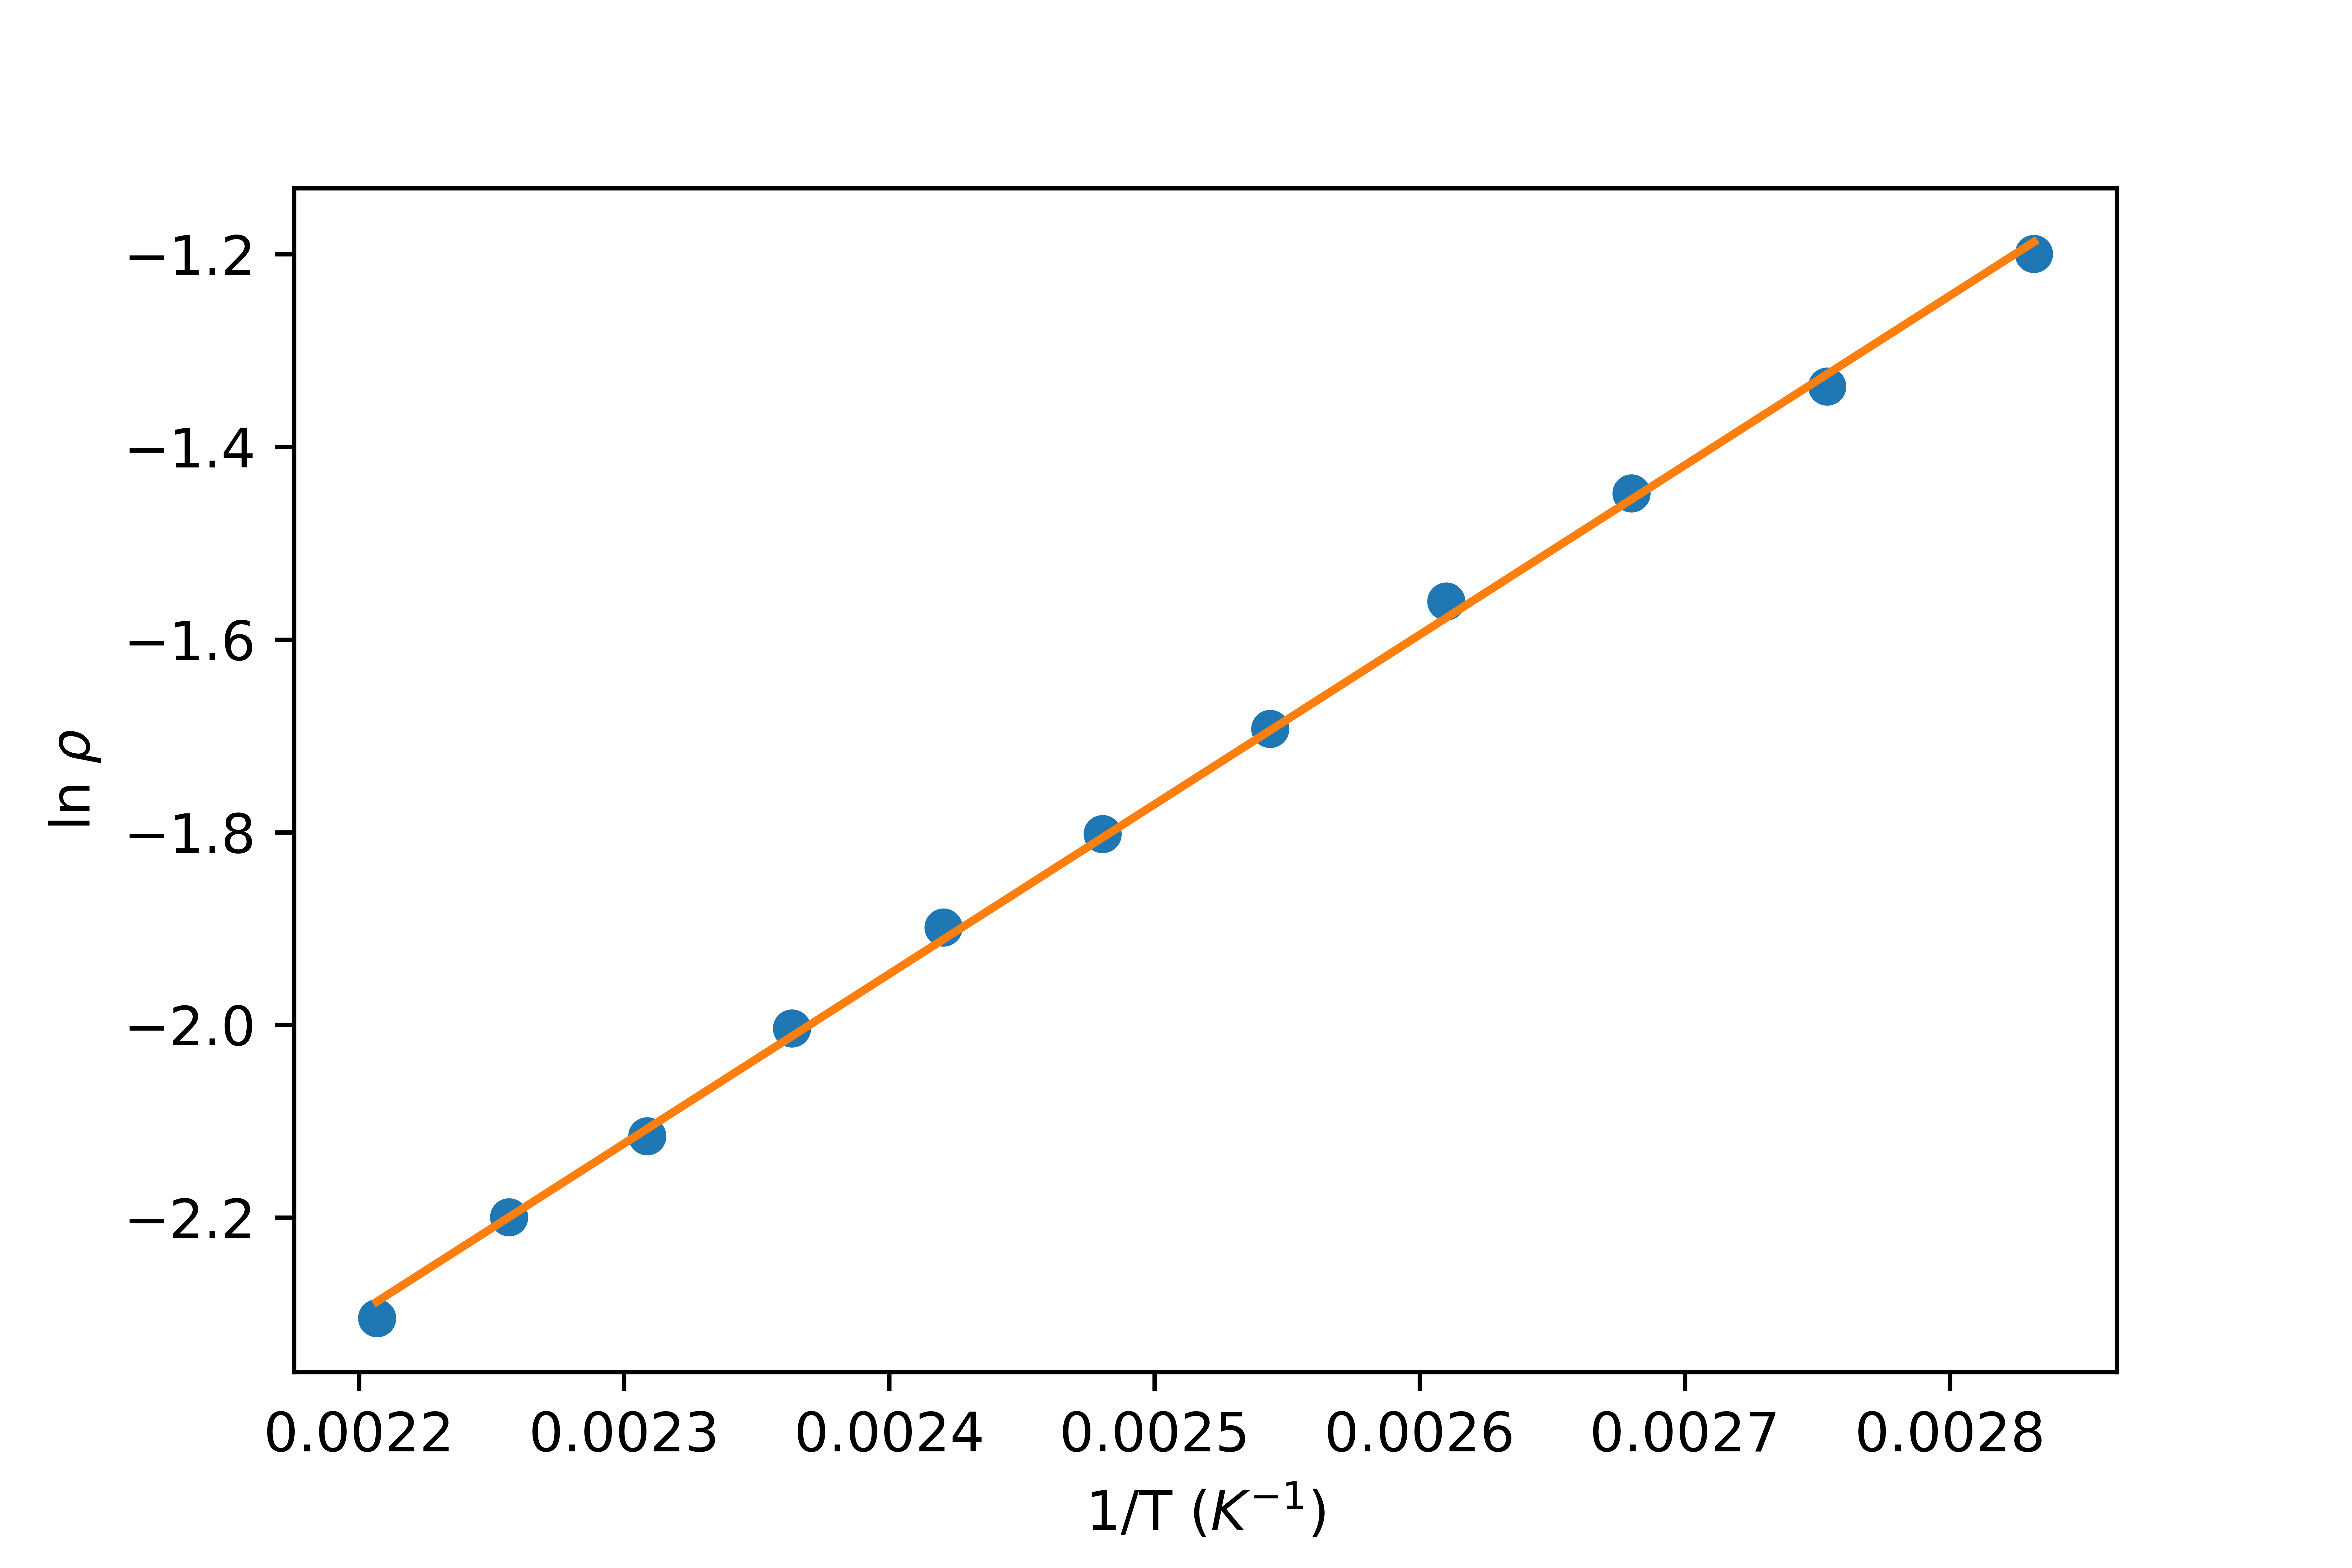
\includegraphics[scale = 0.56]{Figures/plot-temp.png}
    \caption{The $\ln \rho \sim 1/T$ plot for n-Al}
    \label{fig:tempplot}
\end{figure}
\begin{figure}
    \centering
    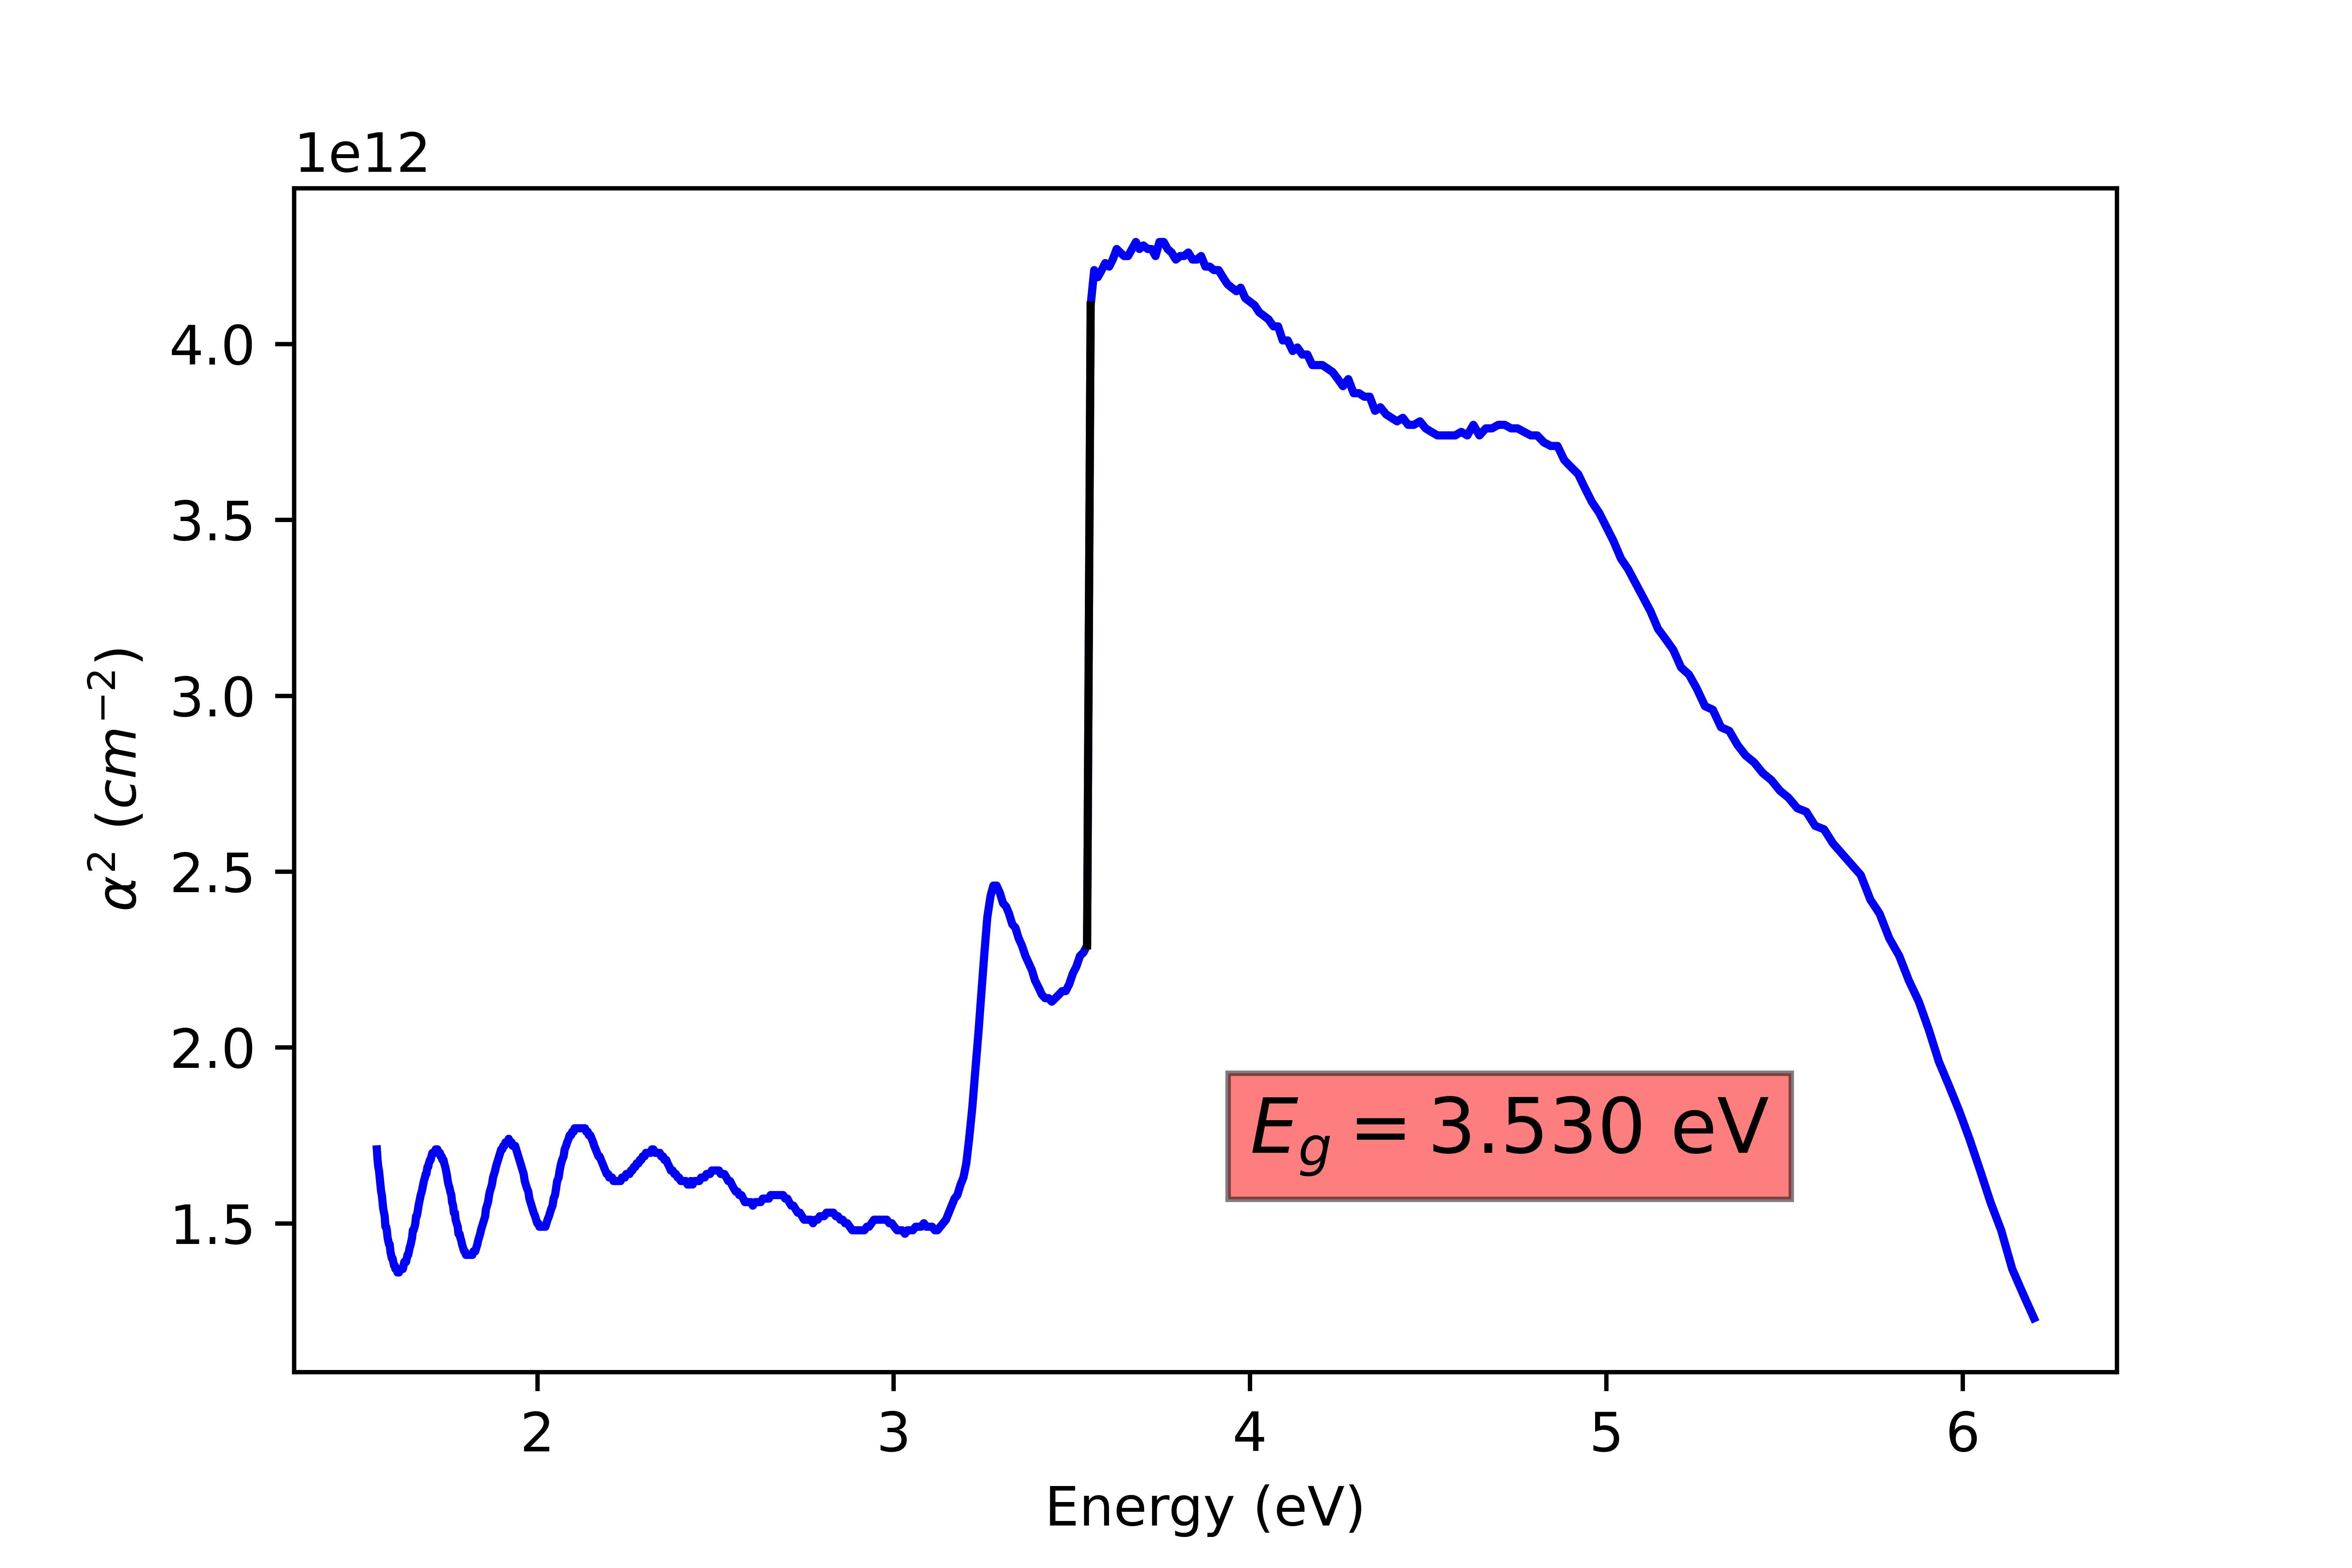
\includegraphics[scale = 0.56]{Figures/plot-1b-ZnO.png}
    \caption{The energy versus absorption coefficient squared plot for ZnO for determination of direct band gap energy}
    \label{fig:znoplot}
\end{figure}
\begin{figure}
    \centering
    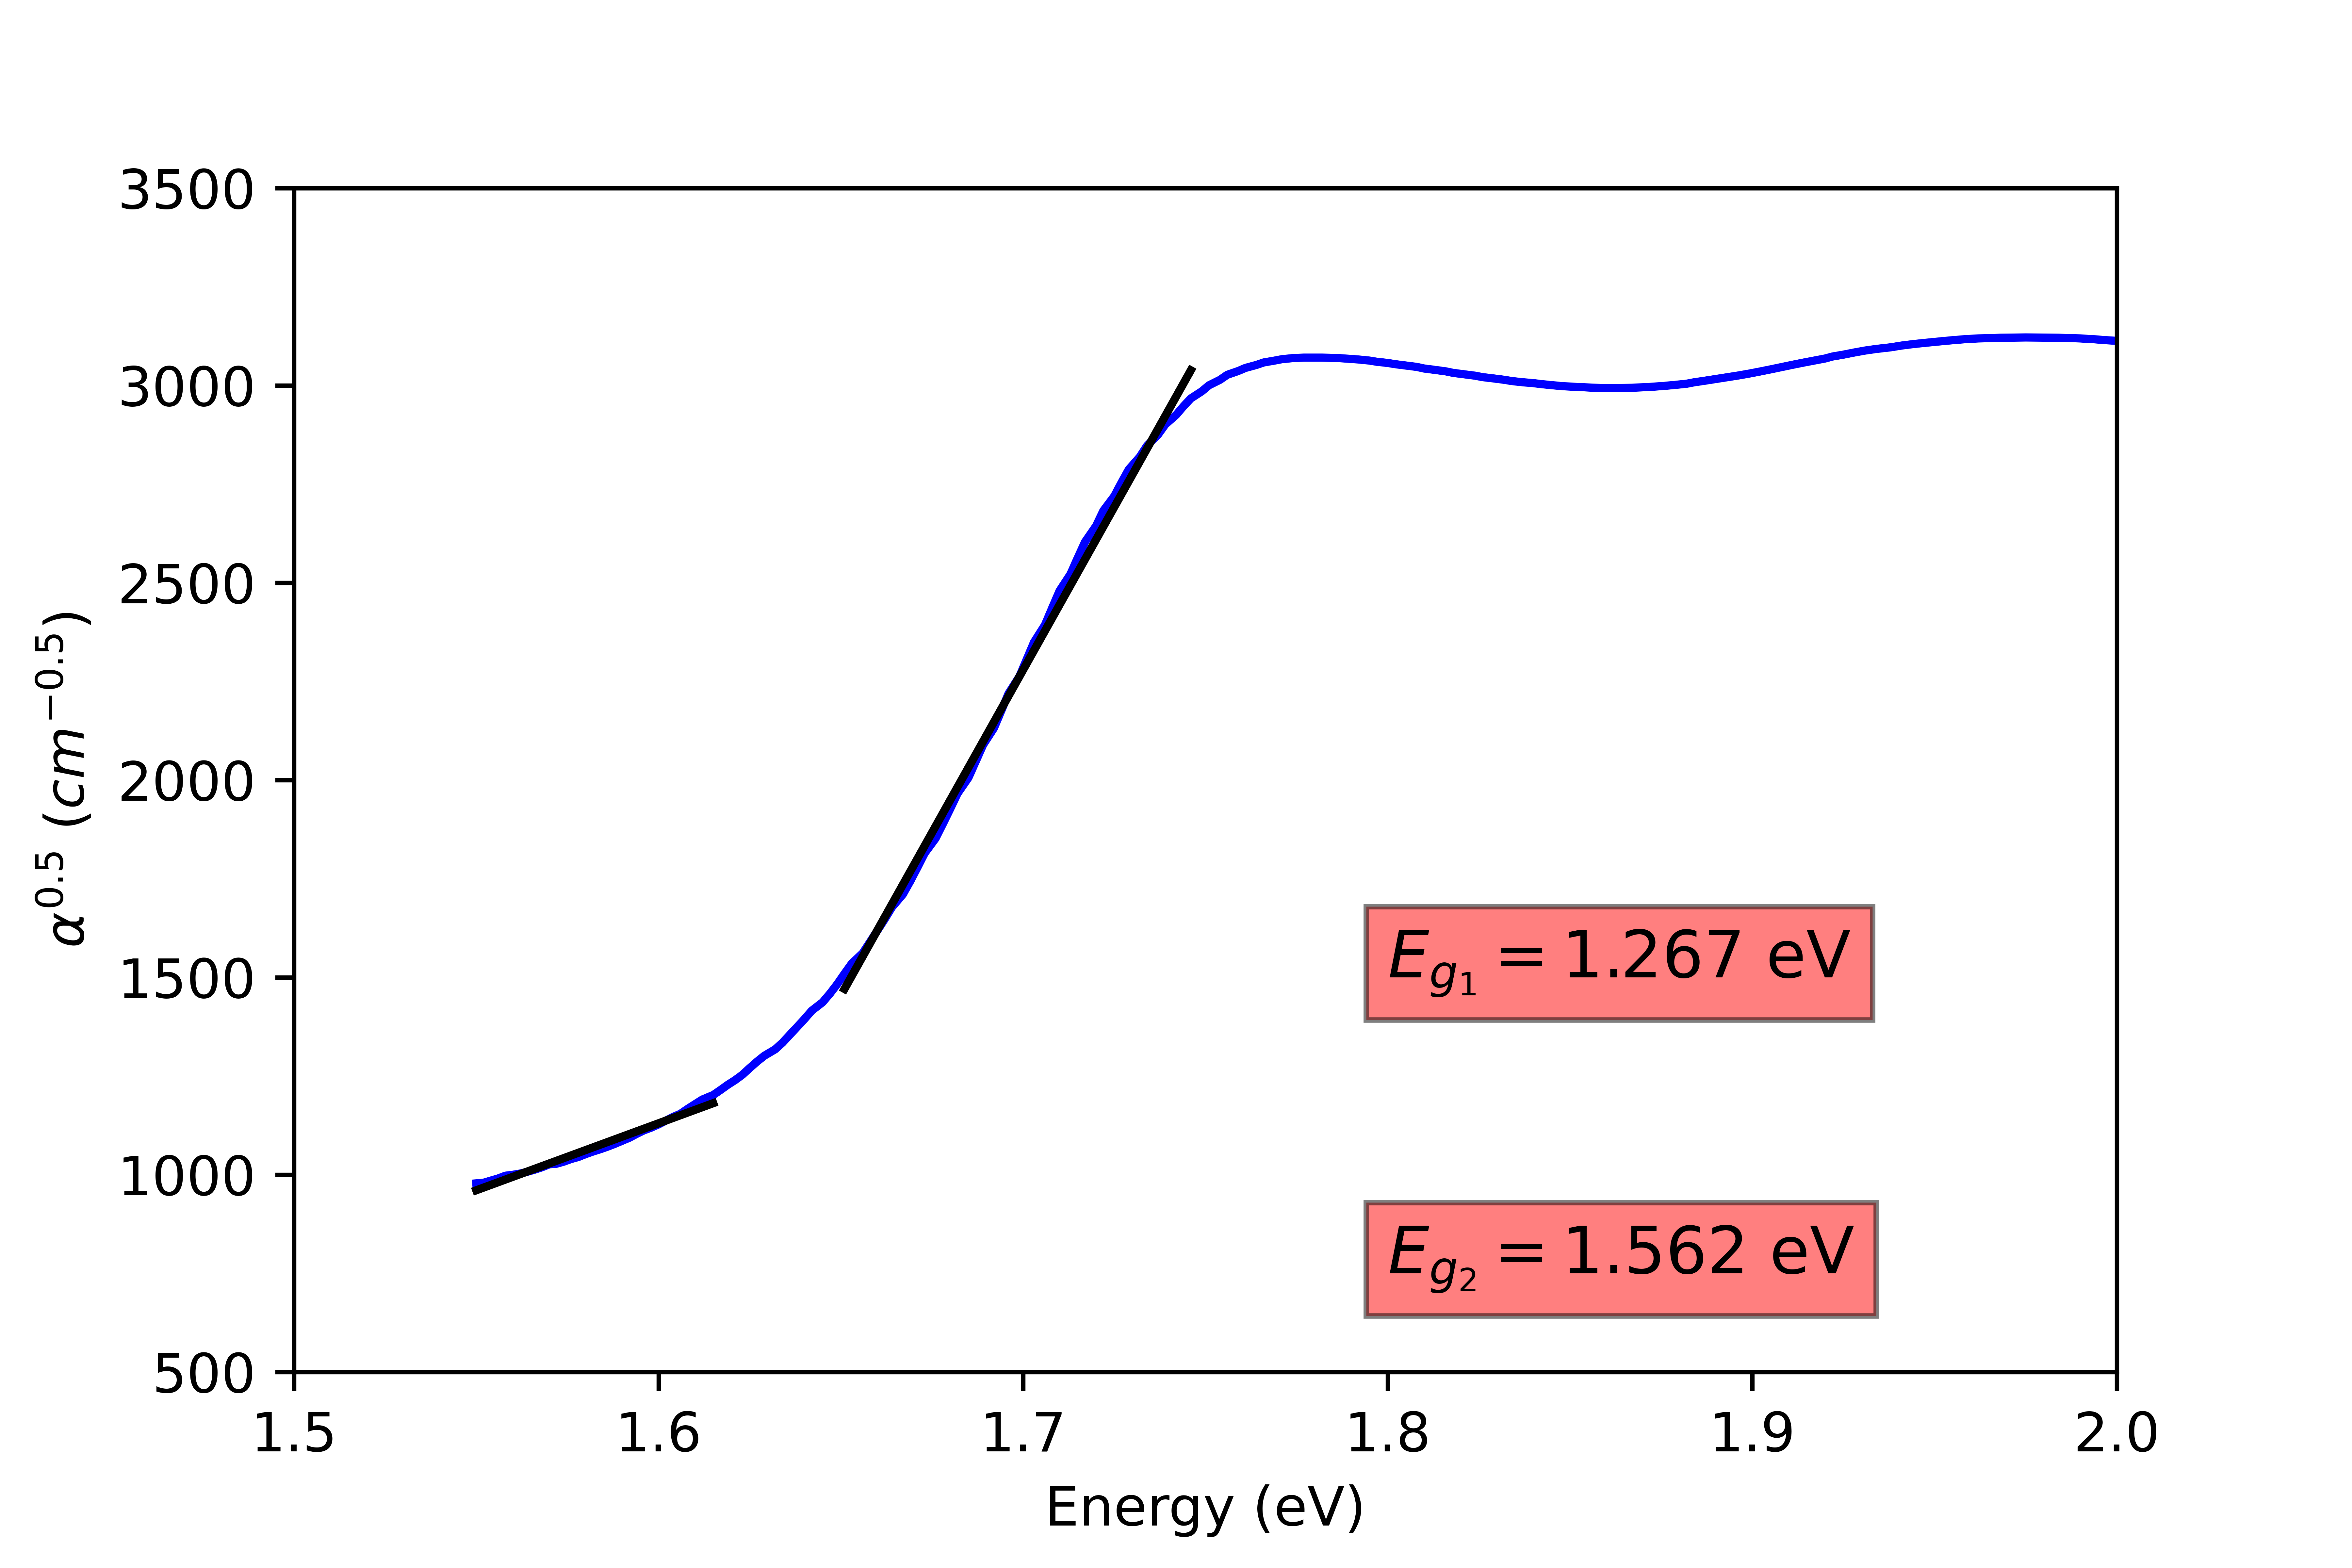
\includegraphics[scale = 0.56]{Figures/plot-1b-Polymer.png}
    \caption{The energy versus square root of absorption coefficient plot for ZnO for determination of indirect band gap energy}
    \label{fig:polymerplot}
\end{figure}
\section{Calculations}
We have
\begin{equation}
\label{rho0}
    \rho_0 = \dfrac{V}{I} 2 \pi S
\end{equation}
And using the correction factor for non-conducting thin-slice case, we have
\begin{equation}
\label{rho}
    \rho = \dfrac{\rho_0}{G_7 (W/S)}
\end{equation}
Further, we know
\begin{equation}
\label{kbt}
    E_g = 2 k_B \dfrac{\ln \rho}{1/T}
\end{equation}
where $k_B$ is the Boltzmann's constant, $k_B = \SI{8.6e-5}{\electronvolt \per \degree}$ and $T$ is temperature in Kelvin. We will use the graph of $1/T \sim V$ to find $E_g$. 
\subsection{Resistivity of n-Silicon}
From figure (\ref{fig:siplot}), the slope of the line is $\SI{104.184}{\ohm}$. Putting the values in equation (\ref{rho0}), we get $\rho_0 = \SI{130.92}{\ohm \centi \metre}$. The value of $G_7 (W/S)$ as calculated from equation (\ref{g7ws}) is $8 \ln 2$. Therefore, using equation (\ref{rho}), we get $\rho_{Si} = \SI{23.60}{\ohm \centi \metre}$.
\subsection{Resistivity of n-Germanium}
From figure (\ref{fig:geplot}), the slope of the line is $\SI{78.2644}{\ohm}$. Putting the values in equation (\ref{rho0}), we get $\rho_0 = \SI{98.35}{\ohm \centi \metre}$. The value of $G_7 (W/S)$ as calculated from equation (\ref{g7ws}) is $8 \ln 2$. Therefore, using equation (\ref{rho}), we get $\rho_{Ge} = \SI{17.74}{\ohm \centi \metre}$.
\subsection{The energy band gap of Germanium}
From figure (\ref{fig:tempplot}), the slope of the line is \SI{1760.316}{\kelvin}. Using equation (\ref{kbt}), we get $E_g = \SI{0.303}{\electronvolt}$. This value is exceptionally different from the expected value and data seems suspect.
\subsection{The energy band gap of ZnO}
From figure (\ref{fig:znoplot}), the equation of the line (in black) is $y = 181999999999989.4x -642535999999962.4.$. This line intersects $X$-axis at $x = \SI{3.530}{\electronvolt}$ which is the $E_g$ value.
\subsection{The energy band gaps of polymer}
From figure (\ref{fig:polymerplot}), the equation of the lines (in black) is $y_1 = 3395.7079287210813x -4302.843449537619.$ and $y_2 = 16502.21642362017x -25774.468514314314.$. These lines intersect $X$-axis at $x_1 = \SI{1.267}{\electronvolt}$ and $x_2 = \SI{1.562}{\electronvolt}$ respectively which are the $E_g$ values.
\section{Error Analysis}
The error in resistivity is given by
\begin{equation}
    d \rho = \sqrt{\Big(\dfrac{\partial \rho}{\partial m} \sigma_{m}\Big)^2 + \Big(\dfrac{\partial \rho}{\partial S} \sigma_{S}\Big)^2}
\end{equation}
where $m$ is the slope of the $V \sim I$ curve for the semiconductor.
Now error in slope, $\sigma_m$ is given by
\begin{equation}
    \sigma_m = \sigma_y \sqrt{\dfrac{s}{\Delta}}
\end{equation}
Here $\sigma_y$ is the least count of $V$ and $s$ and $\Delta$ represent the usual summations in regression analysis.
For the error in temperature variation of resistivity, the error in $E_g$ is just the error in slope of the graph.
\subsection{In the resistivity of n-Silicon}
Putting the values in the above formulae, we get $d \rho_{Si} = \SI{0.5}{\ohm \centi \metre}$.
\subsection{In the resistivity of n-Germanium}
Putting the values in the above formulae, we get $d \rho_{Ge} = \SI{0.3}{\ohm \centi \metre}$.
\subsection{In the energy band gap of Germanium}
As the error in $E_g$ is directly given by the error in slope, we can use the equation directly. Upon doing so, we get, $d E_g = \SI{0.003}{\electronvolt}$.



\section{Results}
\begin{enumerate}
    \item The resitivity of n-Si is given by $\SI[separate-uncertainty=true]{23.6 \pm 0.5}{\ohm \centi \metre}$ which is close to literature value of $\SI{24}{\ohm \centi \metre}$.
    \item The resitivity of n-Ge is given by $\SI[separate-uncertainty=true]{17.7 \pm 0.3}{\ohm \centi \metre}$ which is close to literature value of $\SI{18}{\ohm \centi \metre}$.
    \item The energy band gap for Ge is $E_g = \SI[separate-uncertainty=true]{0.303 \pm 0.003}{\electronvolt}$ which is way off from the literature value of $\SI{0.68}{\electronvolt}$. The possible reasons are discussed in the next section.
    \item The energy band gap for ZnO using UV-Vis spectrophotometer is $E_g = \SI{3.530}{\electronvolt}$.
    \item The energy band gaps for polymer using UV-Vis spectrophotometer is $E_{g_1} = \SI{1.267}{\electronvolt}$ and $E_{g_2} = \SI{1.562}{\electronvolt}$.
\end{enumerate}

\section{Discussions}
\begin{enumerate}
    \item The error analysis for the second part of the experiment was not possible because of not enough data points used to calculate the straight line (especially in the case of ZnO).
    \item The unusually large error in the value of energy band gap for Ge wafer cannot be explained in any way except for suspect data. The data for Aluminium was also suspects which leads to haywire results.
    \item The four-probe method employed in the first part of the experiment to calculate resitivities (and later energy band gap) as several other applications as well like in the field of remote sensing, in production of resistance thermometers in induction hardening process, in the accurate geometry factor estimation and characterization of fuel cells bipolar plates.
\end{enumerate}

\section{Conclusions}
\begin{enumerate}
    \item In most cases, the results so obtained were satisfactory.
    \item There were few cases where the data appeared suspect which were either left (resistivity of n-Al) or calculated as it is (energy band gap of Ge wafer).
\end{enumerate}

\nocite{*}
%\bibliography{bibliography}% Produces the bibliography via BibTeX.

\end{document}
%
% ****** End of file aipsamp.tex ******